\documentclass[]{article}
%\usepackage[a4paper, total={6.5in, 8.5in}]{geometry}

%\usepackage{PRIMEarxiv}

\usepackage{xcolor}
\usepackage{hyperref}
\usepackage{amsmath}
\usepackage{amssymb}
\usepackage{graphicx}
\usepackage{wrapfig}
\usepackage{float}
\usepackage{algorithm}
\usepackage[noend]{algpseudocode}
\usepackage[normalem]{ulem}
\useunder{\uline}{\ul}{}
\usepackage{makecell}
\usepackage{neurips_data_2024}

\graphicspath{/}

\newcommand{\R}{\mathbb{R}}
\newcommand{\EE}{\mathbb{E}}
\newcommand{\N}{\mathbb{N}}
\newcommand{\D}{\mathcal{D}}
\newcommand{\X}{\mathcal{X}}
\newcommand{\Y}{\mathcal{Y}}
\newcommand{\U}{\mathcal{U}}
\newcommand{\LL}{\mathcal{L}}
\newcommand{\test}{\text{test}}
\newcommand{\train}{\text{train}}

%\pagestyle{fancy}
%\thispagestyle{empty}
%\rhead{ \textit{ }} 
%\fancyhead[LO]{Running Title for Header}

\title{Towards Comparable Active Learning}
\author{%
	Anonymous Authors
%	Thorben Werner 
%	\thanks{Institute of Computer Science - Information Systems and Machine Learning Lab (ISMLL)} 
%	\\
%	University of Hildesheim\\
%	Universitätsplatz 1\, 31141 Hildesheim \\
%	\texttt{werner@ismll.de} \\
%	\And
%	Johannes Burchert$^*$ \\
%	University of Hildesheim\\
%	Universitätsplatz 1, 31141 Hildesheim \\
%	\texttt{burchert@ismll.de} \\
%	\And
%	Maximilian Stubbemann$^*$ \\
%	University of Hildesheim\\
%	Universitätsplatz 1, 31141 Hildesheim \\
%	\texttt{stubbemann@ismll.de} \\
%	\AND
%	Lars Schmidt-Thieme$^*$ \\
%	University of Hildesheim\\
%	Universitätsplatz 1, 31141 Hildesheim \\
%	\texttt{schmidt-thieme@ismll.uni-hildesheim.de}
}

\begin{document}


% TODOs nach Priorität
% !! Least-Confident Baseline
% !! "Overfitting on test" für Oracle: Sanity-Check und eventuell komplett streichen
% !! Ergebnis-Tabelle mit nur 3 runs neu berechnen und Unterschiede zeigen
% !! Introduction neu schreiben: Wir brauchen eine klare Benennung der Ziele und bessere Abgrenzung zu anderen papern
% Advantage-Matrix von Ji et. al. neu aufarbeiten. Wo sind die Unterschiede? Ist das CD-Diagramm besser/schlechter?
% Eventuell Batchsize 1 von den anderen Ergebnissen separieren. Der Vergleich macht mehr Sinn, als einfach die Batchsizes zu mitteln
% Infos und Ergebnisse für die syntetischen Datensätze in ein Kapitel bündeln und direkt auf die Contribution beziehen
% Oracle Performance mit einer Zahl benennen: z.B. Da wird ~20% lift zu allen Baselines haben, brauchen wir kein aufwendigeres Oracle
% Contributions neu sortieren und sehr viel ausführlicher beschreiben
% Unsere Rankings mit Literatur vergleichen. Wie anders sind wir? -> Evtl. besten Alg. pro Benchmark sammeln und vergleichen
% Causalitäten checken: Viele Dinge werden einfach genannt, ohne das der Grund richtig eingeführt wird
% "reproducible" als Aufhänger für 50 repeats ist nicht intuitiv
% Fig. 1: Schlechte Performance am Anfang verwirrt nur. Entweder BADGE benutzen, anders plotten, oder im Text in Kontext setzen
% paired-t-test im Critical Difference Diagram herausstellen und die Relevanz für paper zeigen
% Eventuell Honeypot und Diverging Sine direkt in den Contributions nennen
% Oracle Forecast im Appendix erklären 
% Tabelle mit AUCs in den Appendix


\maketitle

\begin{abstract}
Active Learning has received significant attention in the field of machine learning. Its goal is to select the most informative samples for labeling, thereby reducing data annotation costs. 
However, it has been brought to attention multiple times that reported lifts from literature generalize poorly and display high variance, leading to an inconclusive landscape in Active Learning research.
Based on recent insights for reliable evaluation for Active Learning, this work extends experimentation from the commonly used image domain to a wide spectrum of domains.
%This work follows up on recent benchmarking suites for Active Learning, applying the proposed solutions and evaluation protocols to a wide spectrum of domains.
Additionally, we provide an analysis of how many repetitions an Active Learning experiment needs in order to derive conclusive results and propose that previous benchmarks have not met the necessary number of repetitions.
%evidence that existing benchmarks might not have repeated their experiments often enough.
To the best of our knowledge, we propose the first AL benchmark that applies state-of-the-art evaluation on algorithms in 3 major domains: Tabular, Image, and Text as well as synthetic data.
We report empirical results for 10 widely used algorithms on 7 real-world and 2 synthetic datasets and aggregate them into domain-specific and overall rankings of AL algorithms.
\end{abstract}


\section{Introduction}
Deep neural networks (NN) have produced state-of-the-art results on many important supervised learning tasks.
Since Deep NNs usually require large amounts of labeled training data, Active Learning (AL) can be used to instead select the most informative samples out of a large pool of unlabeled data, so that only these samples need to be labeled.
It has been shown that a small labeled set of this nature can be used to train well-performing models \cite{beck2021effective, hu2021towards, li2022empirical, zhou2021towards}. \\
On top of providing a principled way to label unlabeled datasets, active learning is one of the two major approaches besides semi-supervised learning to make deep learning models more data efficient by requiring only a limited set of manually labeled data.
%Both approaches are at their core orthogonal and can freely be combined and therefore we should continue our research efforts for both approaches. \\
In the last decade, many different algorithms for AL have been proposed.
Even though, almost every method has reported lifts over all its predecessors,
\footnote{Out of all considered algorithms for this paper, only BALD \cite{gal2017deep} did not claim a new SOTA performance in their result section.}
AL research faces four central difficulties:
{\let\thefootnote\relax\footnotetext{Code available at: anonymous}}
%\let\thefootnote\relax\footnotetext{Code available at: \url{https://github.com/wernerth94/comparable-active-learning}}
(i) The experiments are often carried out on different datasets and model architectures, hindering direct comparison,
(ii) generalize poorly across different domains,
(iii) the reported results can be subject to very high variance across restarts and
(iv) are not always compared against important baselines like margin sampling \cite{wang2014new}.
While multiple benchmark suites have been proposed to solve (i), to the best of our knowledge, we are the first to report results on all 3 data domains of tabular, image and text.
Additionally, we provide synthetic datasets to highlight principled shortcoming of existing AL algorithms.
Regarding (ii) and (iii), \cite{zhou2021towards} has pointed out severe inconsistencies in results of AL papers in recent years. 
They conducted a meta analysis of reported results of several different AL algorithms and found that all considered algorithms only provided significant lifts in their own original papers, while following literature reported performances no better that uncertainty sampling, or in some cases no better than random sampling for the same algorithm (\cite{zhou2021towards} Appendix A).
These outlined issues lead to an inconclusive landscape of AL algorithms, where the vast majority of reported lifts are neither statistically significant, nor prove to be generalizable.
This makes it very hard to identify the best AL algorithm, or even identifying state-of-the-art algorithms.
In this work we propose an evaluation protocol that was designed to handle the high variance in the performances of AL algorithms as well as being fully controllable regardless of the combination of dataset, model and AL algorithm. 
We base our work largely on \cite{ji2023randomness}, following their guidelines for a reliable evaluation of AL algorithms, while extending the number of evaluated data domains from 1 to 5. \\
We focus on pool-based AL where a pool of unlabeled samples is fixed at the start of each experiment and one or more samples are chosen sequentially.
In addition to the default scenario of selecting a batch of samples every iteration we incorporate the single sample case into our benchmark.
Batched algorithms (and benchmarks) do not have a principled advantage over single-sample AL except for speed of computation.
The problem of optimizing a portfolio of unlabeled samples in each iteration is more complicated to solve and the algorithms have systematically less information per sample to work with leading to a generally worse performance, that impacts some algorithms more than others. 
%In Fig. \ref{fig:batch_vs_single} we present a comparison of Badge \cite{ashdeep} and Coreset\cite{sener2017active}, in the batch and single-sample setting.
%Even though both algorithms were designed for batch sampling, both perform better in the single-sample setting.
We propose single-sample AL as an important tool to identify the best acquisition function, rather than the best combination of acquisition function and diversity regularization. \\
%\begin{figure}
%    \centering
%    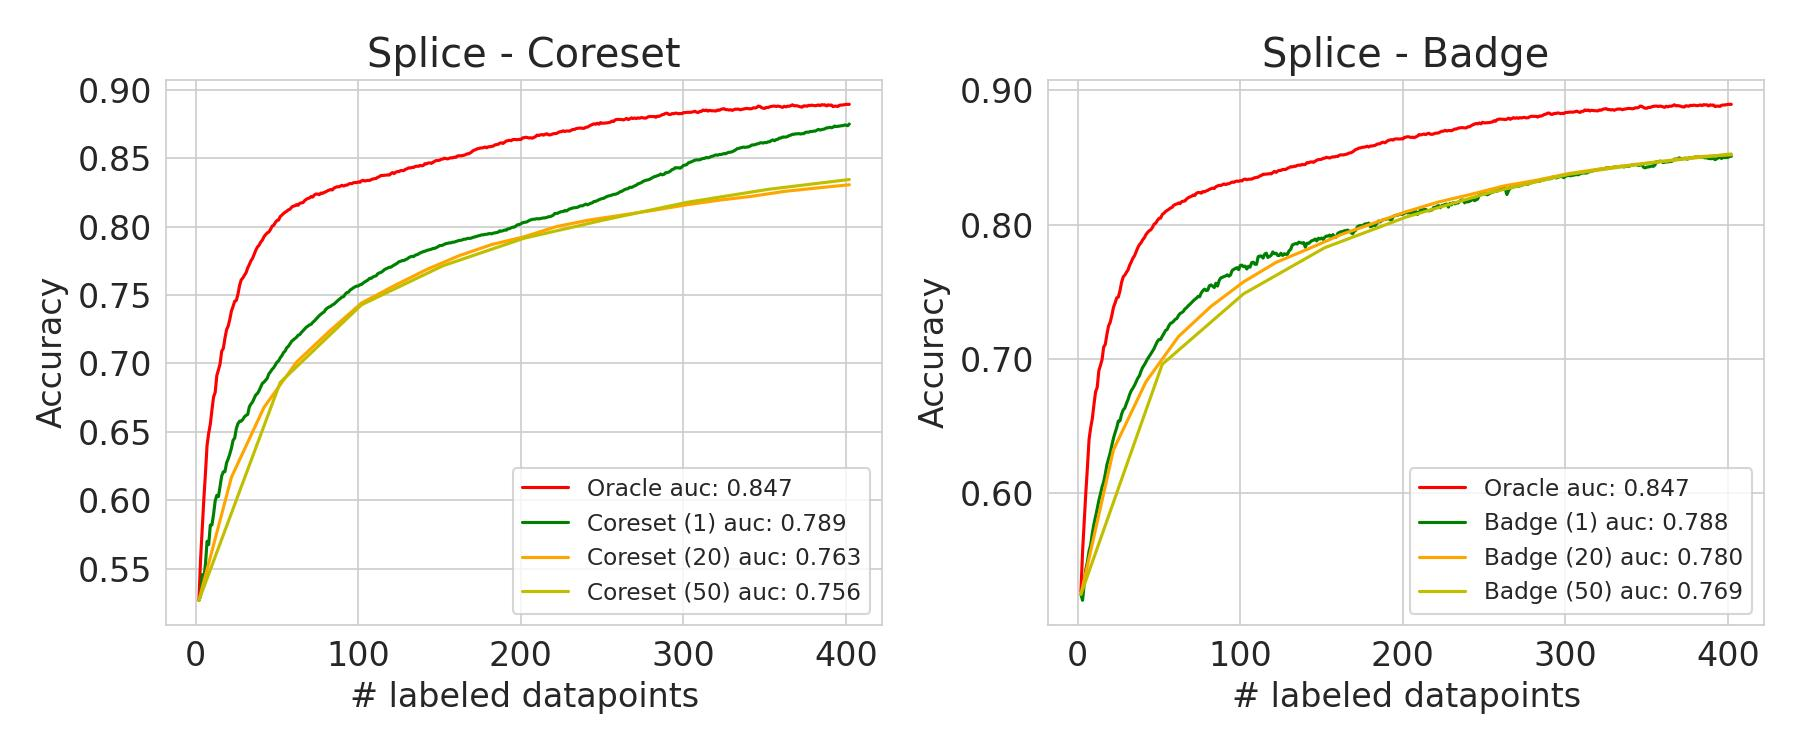
\includegraphics[width=\linewidth]{img/ablation_batch_single}
%    \caption{Comparison of single-sample vs. batch selection for two acquisition functions that were specifically designed for batch selection. Even when designed for batch selection, acquisition functions tend to perform better in the single sample setting.}
%    \label{fig:batch_vs_single}
%\end{figure}
Table \ref{tab:benchmark_comparison} shows a feature comparison between our proposed benchmark and several existing benchmarks in the literature. 
We offer our datasets in two versions - normal and encoded.
An encoded dataset was pre-encoded by an self-supervised encoder model, providing a different use case for active learning.
Our synthetic and text datasets (which use word embeddings in the normal setting) are exempt from this, bringing our total dataset count to 14 across 5 domains (Tabular, Image, Text, Synthetic, Encoded).
\begin{table}
	\centering
        \caption{Comparison of our benchmark with the existing literature. Oracle curves serve as an approximation of the best possible AL algorithm. Including the encoded versions of our datasets we reach 14 datasets. "Semi" indicates whether the paper is employing any form of self- or semi-supervised learning. A "-" for repetitions means that we could not determine how often each experiment is repeated in the respective framework.}
	\label{tab:benchmark_comparison}
	\resizebox{\columnwidth}{!}{
\begin{tabular}{lccccllllcl}
\hline
Paper & Sampling & \#Data & \#Alg & \multicolumn{1}{l}{Img} & Txt & Tab & Synth & Semi & Oracle & Repetitions \\ \hline
\multicolumn{1}{l|}{Beck et al. \cite{beck2021effective}} & batch & 4 & 7 & \checkmark & - & - & - & - & - & - \\
\multicolumn{1}{l|}{Hu et al. \cite{hu2021towards}} & batch & 5 & 13 & \checkmark & \checkmark & - & - & - & - & 3 \\
\multicolumn{1}{l|}{Zhou et al. \cite{zhou2021towards}} & batch & 3 & 2 & \checkmark & \checkmark & - & - & - & \checkmark & 5 \\
\multicolumn{1}{l|}{Zhan et al. \cite{zhan2021comparative}} & sngl+batch & 35 & 18 & - & - & \checkmark & \checkmark & - & \checkmark & 10-100 \\
\multicolumn{1}{l|}{Munjal et al. \cite{munjal2022towards}} & batch & 2 & 8 & \checkmark & - & - & - & - & - & 3 \\
\multicolumn{1}{l|}{Li et al. \cite{li2022empirical}} & batch & 5 & 13 & \checkmark & - & - & - & \checkmark & - & - \\
\multicolumn{1}{l|}{Ji et al. \cite{ji2023randomness}} & batch & 3 & 8 & \checkmark & - & - & - & - & - & - \\
\multicolumn{1}{l|}{Luth et al. \cite{luth2024navigating}} & batch & 4 & 5 & \checkmark & - & - & - & \checkmark & - & 3 \\
\multicolumn{1}{l|}{\textbf{Ours}} & sngl+batch & 9(14) & 10 & \checkmark & \checkmark & \checkmark & \checkmark & \checkmark & \checkmark & 50 
\end{tabular}
}
\end{table}

\subsection*{Contributions}
\begin{enumerate}
	\item Evaluation of Active Learning algorithms on datasets from 5 different domains
	\item Two novel synthetic datasets that highlight principled shortcomings of existing AL algorithms
	\item Efficient and performant algorithm for an oracle that can be constructed greedily and does not rely on search
        \item Evidence that previous works might have not repeated their experiments often enough to provide conclusive results
\end{enumerate}


%%%%%%%%%%%%%%%%%%%%%%%%%%%%%%%%%%%%%%%%%%%%%%%%%%%%%%%%%%%%%%%%%%%%%%%%%%%%%%%%%%
\section{Problem Description}
Given two spaces $\X, \Y$, $n=l+u$ data points with $l \in \mathbb{N}$ labeled examples $\mathcal{L} = \{(x_1, y_1),\ldots, (x_l,y_l)\}$, $u \in \mathbb{N}$ unlabeled examples $\mathcal{U} = \{x_{l+1},\ldots,x_{n}\}$, a model $\hat y: \X \to \Y$, a budget $\mathbb{N} \ni b \le u$ and an annotator $A: \mathcal{X} \to \mathcal{Y}$ that can label $x$ (we consider only hard labels in the one-hot format). 
We call $x \in \mathcal{X}$, $y \in \mathcal{Y}$ predictors and labels respectively where $(x,y)$ are drawn from an unknown distribution $\rho$. 
Find an acquisition function $\Omega: \U^{(i)},\LL^{(i)} \mapsto x^{(i)} \in \U^{(i)}$ that iteratively selects the next unlabeled point $x^{(i)}$ for labeling
\begin{align*}
	\LL^{(i+1)} &\gets \LL^{(i)} \cup \{\left(x^{(i)}, A(x^{(i)})\right)\} \\
	\U^{(i+1)} &\gets \U^{(i)} \setminus x^{(i)} %, i \in 1{:}B
\end{align*}
with $\U^{(0)} = \operatorname{seed}(\U, s)$ and $\LL^{(0)} = \{\left(\U^{(0)}, A(\U^{(0)})\right)\}$, where $\operatorname{seed}(\U, s)$ selects $s$ points per class for the initial labeled set. \\
So that the average expected loss $\ell: \mathcal{Y} \times \mathcal{Y} \to \mathbb{R}$ of a machine learning algorithm fitting $\hat y^{(i)}$ on the respective labeled set $\LL^{(i)}$ is minimal: 
$$\min \quad \frac{1}{B} \sum\limits_{i=0}^B \mathbb{E}_{(x,y) \sim \rho} \ell(y, \hat y^{(i)})$$

%%%%%%%%%%%%%%%%%%%%%%%%%%%%%%%%%%%%%%%%%%%%%%%%%%%%%%%%%%%%%%%%%%%%%%%%%%%%%%%%%%
%%%%%%%%%%%%%%%%%%%%%%%%%%%%%%%%%%%%%%%%%%%%%%%%%%%%%%%%%%%%%%%%%%%%%%%%%%%%%%%%%%
%%%%%%%%%%%%%%%%%%%%%%%%%%%%%%%%%%%%%%%%%%%%%%%%%%%%%%%%%%%%%%%%%%%%%%%%%%%%%%%%%%
\section{Related Work}
Multiple benchmark suites have already been proposed for Active Learning:
The authors of \cite{beck2021effective}, \cite{munjal2022towards}, \cite{li2022empirical}, \cite{ji2023randomness} and \cite{luth2024navigating} focus exclusively on batch AL in the image domain.
While \cite{beck2021effective} discuss a new metric to measure AL performance, which they call ``Label Efficiency'' and provide experiments on many common configurations of data preparation, model training, and other hyperparameters, \cite{li2022empirical} focuses on combined approaches of AL and semi-supervised learning.
The authors of \cite{hu2021towards} study models that are trained on actively learned datasets in the image and text domain.
They test for several different properties of the models including robustness, response to compression techniques and final performance.
\cite{zhou2021towards} proposed an oracle algorithm for AL that uses Simulated Annealing search to approximate a solution for the optimal subset of labeled data.
Additionally, they study the generalization behavior of subsets of labeled data in the text an image domain.
The two closest related works to this benchmark are \cite{ji2023randomness} and \cite{luth2024navigating}, who also discussed the problems of evaluating AL algorithms under many forms of variance.
We largely adapt the proposed guidelines of \cite{ji2023randomness} and extend their work to multiple domains, batch sizes and comparisons. 
This work also pays attention to the so-called "pitfalls" of AL evaluation mentioned in \cite{luth2024navigating} with the exception of P1 - Controlling the data distribution of the tested datasets.
We leave this aspect for future versions of this benchmark. \\
Two preceding benchmarks have also proposed an oracle algorithm to find a near-optimal labeled set $\LL$, however, both algorithms rely on search and are for that reason considerably slower than our proposed greedy oracle.

%%%%%%%%%%%%%%%%%%%%%%%%%%%%%%%%%%%%%%%%%%%%%%%%%%%%%%%%%%%%%%%%%%%%%%%%%%%%%%%%%%
%%%%%%%%%%%%%%%%%%%%%%%%%%%%%%%%%%%%%%%%%%%%%%%%%%%%%%%%%%%%%%%%%%%%%%%%%%%%%%%%%%
%%%%%%%%%%%%%%%%%%%%%%%%%%%%%%%%%%%%%%%%%%%%%%%%%%%%%%%%%%%%%%%%%%%%%%%%%%%%%%%%%%
\section{Methodology}

%%%%%%%%%%%%%%%%%%%%%%%%%%%%%%%%%%%%%%%%%%%%%%%%%%%%%%%%%%%%%%%%%%%%%%%%%%%%%%%%%%
\subsection{Evaluation Protocol}\label{sec:evaluation}
Following \cite{zhou2021towards}, the quality of an AL algorithm is evaluated by an ``anytime protocol" that incorporates classification performance at every iteration, as opposed to evaluating final performance after the budget is exhausted.
We employ the normalized area under the accuracy curve (AUC):
\begin{equation}\label{eq:auc}
	\operatorname{AUC}(\D_\test, \hat y, B) := \frac{1}{B} \sum_{i=1}^{B} \operatorname{Acc}(\D_\test, \hat y^{(i)})
\end{equation}
The AUC incorporates performance in early stages (low budget) as well as capabilities to push the classifier in later stages (high budget).
AL algorithms have to perform well in both scenarios. 
\\ [1mm]
Since AUC is still influenced by the budget, we define a set of rules to set this hyperparameter upfront, so that we are not favoring a subset of algorithms by handcrafting a budget.
In this work, we choose the budget per dataset to be the first point at which one of 2 stopping conditions apply: (i) an algorithm (except Oracle) manages to reach 99\% of the full-dataset-performance (using the smallest query size) or (ii) the best algorithm (except oracle) did not improve the classifier's accuracy by at least 2\% in the last 20\% of iterations. \\ [1mm]
%\footnote{Since we only consider single-sample AL, increasing the budget comes at a high computational cost. Therefore we could not freely increase the budget above 2000.} 
To mimic the leave-one-out protocol for cross-validation, we will restart each experiment multiple times.
Each restart retains the train/test split (often given by the dataset itself), but introduces a new validation split that is sampled from the entire dataset (not just $\LL$).

%%%%%%%%%%%%%%%%%%%%%%%%%%%%%%%%%%%%%%%%%%%%%%%%%%%%%%%%%%%%%%%%%%%%%%%%%%%%%%%%%%
\subsection{Why we need 50 restarts}\label{sec:restarts}
To evaluate how many restarts are necessary to obtain conclusive and reproducible results in an AL experiment, we set the number of restarts fore margin sampling on the Splice dataset to 100.
This allows us firstly, to obtain a very strong estimation of the "true" average performance of margin sampling on this dataset and secondly, to draw subsets from this pool of 100 runs.
Setting the size of our draws to $\alpha$ and sampling uniformly, we can approximate a cross-validation process with $\alpha$ restarts.
Each of these draws can be interpreted as a reported result in AL literature where the authors employed $\alpha$ restarts.
%We provide evidence in Fig. \ref{fig:restarts} that previous works might not have evaluated their experiments with a sufficient number of restarts.
Figure \ref{fig:restarts} shows the "true" mean performance of margin sampling (green) in relation to random sampling (black) and the oracle performance (red).
We display 5 random draws of size $\alpha$ in blue.
We can observe that even for a relatively high number of restarts the variance between the samples is extremely high, resulting in some performance curves being worse that random and some being significantly better.
When setting $\alpha = 50$ we observe all samples to converge close to the true mean performance. 
For that reason, we employ 50 restarts of every experiment in this work.
\begin{figure}
        \hspace{-20mm}
	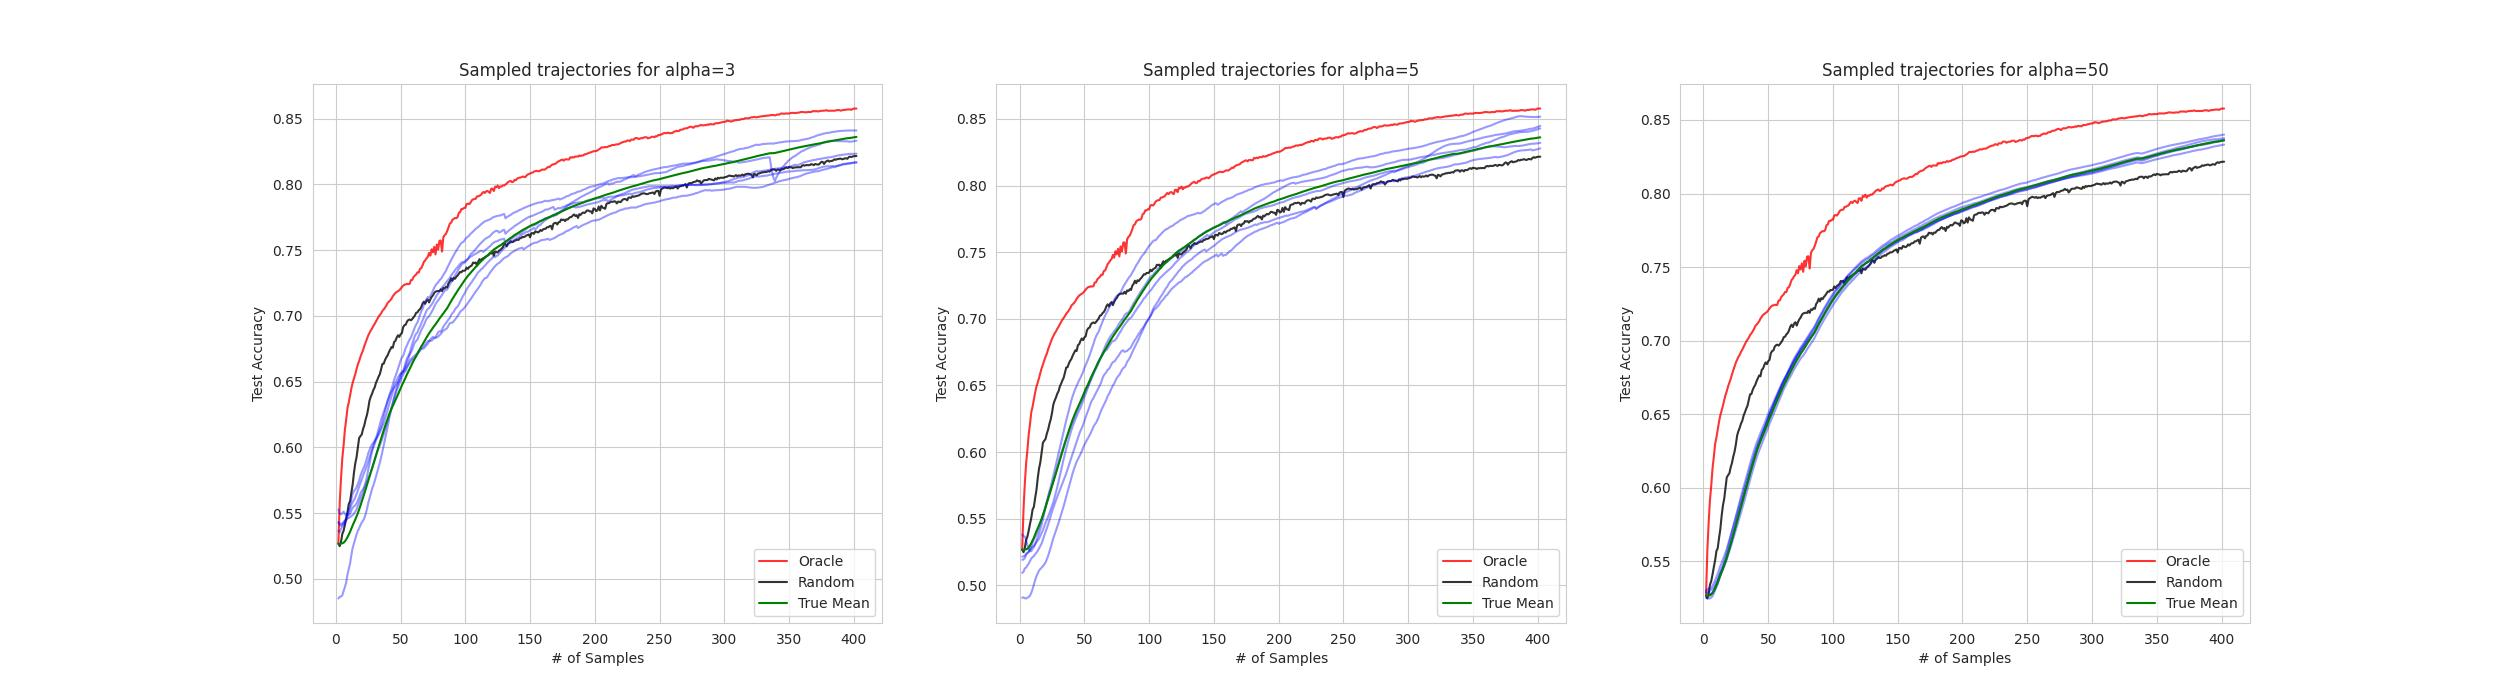
\includegraphics[width=1.24\linewidth]{img/ablation_restarts}
	\caption{Random draws from a pool of 100 runs for margin sampling on the Splice dataset with different numbers of repetitions ($\alpha=\{5,10,50\}$). Green curves are the mean performance of all 100 runs, while the samples are blue. Even with 5 or 10 repetitions, we can observe that single draws for margin sampling display below-random performance (black), while the true mean should be above random.}
	\label{fig:restarts}
\end{figure}


%%%%%%%%%%%%%%%%%%%%%%%%%%%%%%%%%%%%%%%%%%%%%%%%%%%%%%%%%%%%%%%%%%%%%%%%%%%%%%%%%%
\subsection{Seeding vs. Restarts}\label{sec:reproducibility}
Considering the high computational cost of 50 repetitions, another approach to ensure reproducibility would be to reduce the amount of variance in the experiment by keeping as many subsystems (weight initialization, data splits, etc.) as possible fixed with specialized seeding. \\
We describe a novel seeding strategy in Appendix \ref{app:seeding_strategy} that creates 3 separate Random Number Generators (RNG) based on 3 different seeds.
In short, we introduce three different seeds: $s_\Omega$ for the AL algorithm, $s_\mathcal{D}$ for dataset splitting and mini-batch sampling, and $s_\theta$ for model initialization and sampling of dropout masks.
Unless stated otherwise, we will keep $s_\Omega$ fixed, while $s_\mathcal{D}$ and $s_\theta$ are incremented by 1 between restarts to introduce stochasticity into our framework.
While this seeding strategy is capable of controlling the amount variance in the experiment, previous works have noted that an actively sampled, labeled set does not generalize well between model architectures or even different initializations of the same model (\cite{zhou2021towards, lowell2018practical}), reducing its value in practice and providing a bad approximation of the quality of an AL algorithm.
Hence, we opt for letting the subsystems vary (by increasing $s_\mathcal{D}$ and $s_\theta$) and combine that with a high number of restarts to obtain a good average of the generalization performance of each AL algorithm. \\
Where a high number of restarts is computationally not feasible, we advise to additionally keep either $s_\mathcal{D}$ or $s_\theta$ (or both) fixed.


%%%%%%%%%%%%%%%%%%%%%%%%%%%%%%%%%%%%%%%%%%%%%%%%%%%%%%%%%%%%%%%%%%%%%%%%%%%%%%%%%%
\subsection{Datasets}\label{sec:datasets}
A detailed description of the preprocessing of each dataset can be found in Appendix \ref{app:hyperparameters}. \\ [1mm]
\textbf{Tabular:}
AL research conducted on tabular data is sparse (only \cite{ashdeep} from the considered baseline papers). 
We, therefore, introduce a set of tabular datasets that we selected according to the following criteria:
(i) They should be solvable by medium-sized models in under 1000 samples, (ii) the gap between most AL algorithms and random sampling should be significant (potential for AL is present) and (iii) the gap between the AL algorithms and our oracle should also be significant (research on these datasets can produce further lifts).
We use \textbf{Splice}, \textbf{DNA} and \textbf{USPS} from LibSVMTools \cite{libsvmtools}.\\
\textbf{Image:}
We use \textbf{FashionMNIST} \cite{xiao2017fashion} and \textbf{Cifar10} \cite{krizhevsky2009learning}, since both are widely used in AL literature.\\
\textbf{Text:}
We use \textbf{News Category} \cite{misra2022news} and \textbf{TopV2} \cite{chen-etal-2020-low-resource}.
Text datasets have seen less attention in AL research, but most of the papers that evaluate on text (\cite{hu2021towards}, \cite{zhou2021towards}) use at least one of these datasets.\\ [1mm]
%
We would like to point out that these datasets are selected for speed of computation (both in terms of number of features and necessary budget to solve the dataset). 
However, similar to our argumentation for picking smaller classifiers, we are solely focused on comparing different AL algorithms in this paper and do not aim to develop novel classification models on these datasets.
Our assumption is that a well-performing algorithm in our benchmark will also generalize well to larger real-world datasets, because we included multiple different data domains and classifier sizes in our experiments. \\ [1mm]
Adapting the experimental setting from \cite{hacohen2022active}, we offer all our datasets in the un-encoded (normal) setting as well as pre-encoded by a fixed embedding model that was trained by unsupervised contrastive learning. 
The text datasets are an exception to this, as they are only offered in their encoded form.
The pre-encoded datasets enable us to test single-sample algorithms on more complex datasets like Cifar10 and FashionMnist.
They also serve the purpose of investigating the interplay between self-supervised learning techniques and AL, as well as alleviating the cold-start problem described in \cite{luth2024navigating} as they require a way smaller seed set.
The classification model for every encoded dataset is a single linear layer with softmax activation.
The embedding model was trained with the SimCLR \cite{chen2020simple} algorithm adopting the protocol from \cite{hacohen2022active}. 
%For Cifar10 and FashionMnist we adapt the reported hyperparameters from \cite{hacohen2022active} and for the tabular datasets we use random search to optimize the hyperparameters.
To ensure that enough information from the data is encoded by our embedding model, the quality of embeddings during pretext training was measured after each epoch.
We attached a linear classification head to the encoder, fine-tuned it to the data and evaluated this classifier for test accuracy, mirroring our AL setup for embedded datasets. 
The checkpoint of each encoder model will be provided together with the framework. \\ [1mm]
\textbf{Synthetic Data}
Existing AL algorithms can broadly be categorized into two types, uncertainty \cite{wang2014new, gal2017deep} - and geometric-approaches \cite{sener2017active, hacohen2022active, ashdeep}. 
Both types have principled shortcomings in terms of the utilized information that makes them unsuitable for certain data distributions.
To test for these shortcomings, we created two synthetic datasets, namely "Honeypot" and "Diverging Sine", that are hard to solve for methods focused on the classifier's decision boundary or data clustering respectively. 
To avoid algorithms memorizing these datasets they are generated during the experiment, depending on $s_\D$. \\
\begin{figure}[H]
	\centering
	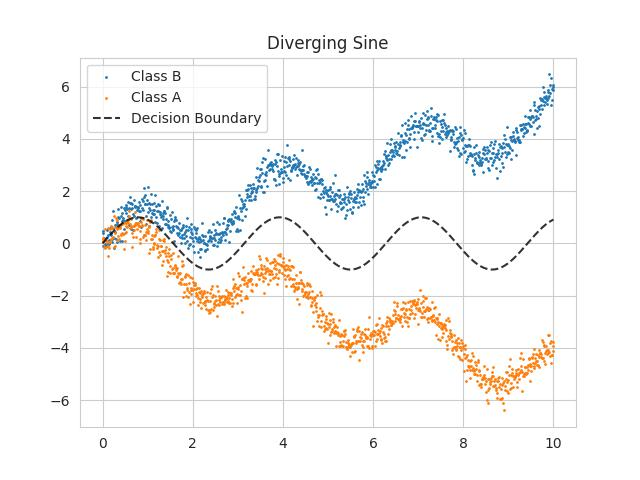
\includegraphics[width=0.4\linewidth]{img/diverging_sin.jpg}
	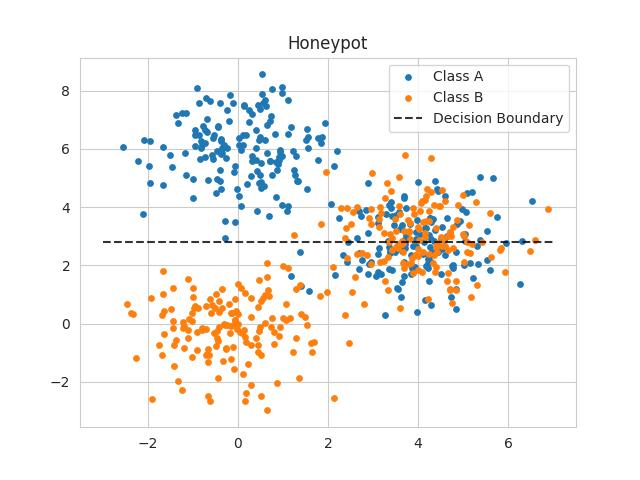
\includegraphics[width=0.4\linewidth]{img/honeypot.jpg}
	\caption{Synthetic "Honeypot" and "Diverging Sine" datasets. The decision boundary is not part of the dataset and serves only as a visual guide.}
        \label{fig:synthDataAppendix}
\end{figure}
Honeypot creates to two easy to distinguish clusters with 150 samples each and one overlapping "honeypot" that represents a noisy region of the dataset with potentially miss-labeled, miss-measured or generally adverse samples.
This honeypot contains 150 samples of each class, creating a balance of 50\% beneficial samples and 50\% adverse samples in the dataset.
The honeypot is located on the likely decision boundary of a classifier that is trained on the beneficial samples to maximize its negative impact on purely uncertainty based acquisition functions.
Diverging Sine samples the datapoints for each class from two diverging sinusoidal functions that are originating from the same y-intercept.
This creates a challenging region one the left hand side, where a lot of datapoints need to be sampled and an easy region on the right hand side, where very few datapoints are enough. 
The repeating nature of a sin function encourages diversity based acquisition functions to equally sample the entire length, drastically oversampling the right hand side of the dataset.
Each class has 500 datapoints. \\ [1mm]
Every dataset has a fixed size for the seed set of 1 sample per class, with the only exceptions being un-encoded FashionMnist and Cifar10 with 100 examples per class to alleviate the cold-start problem in these complex domains. 

%%%%%%%%%%%%%%%%%%%%%%%%%%%%%%%%%%%%%%%%%%%%%%%%%%%%%%%%%%%%%%%%%%%%%%%%%%%%%%%%%%
\subsection{Classification Model}\label{sec:choosing_the_classifier}
\begin{wraptable}{R}{0.65\textwidth}
    \vspace{-0.7cm}
    \caption{Overview of available batch sizes for each dataset}
    \vspace{0.1cm}
    \label{tab:batch_sizes}
    \begin{tabular}{l|c|c|c|c|c|c|c|c}
                    & B & 1 & 5 & 20 & 50 & 100 & 500 & 1000 \\
         \hline
        Enc. DNA    & 40 & o & o &&&&& \\
        Honeypot    & 60 & o & o &&&&& \\
        Diverging Sine& 60 & o & o &&&&& \\
        Enc. Splice & 100 & o & o & o & o &&&\\
        TopV2       & 200 & o & o & o & o &&& \\
        Splice      & 400 & o & o & o & o & o && \\
        DNA         & 300 & o & o & o & o & o && \\
        USPS        & 400 & o & o & o & o & o && \\
        Enc. Cifar10& 450 & o & o & o & o & o && \\
        Enc. FMnist & 500 & o & o & o & o & o && \\
        Enc. USPS   & 600 & o & o & o & o & o && \\
        News        & 3K &&& o & o & o & o &\\
        FMnist      & 10K &&&&&& o & o\\
        Cifar10     & 10K &&&&&& o & o \\
    \end{tabular}
    \vspace{-0.35cm}
\end{wraptable}
The model $\hat y$ can be trained in two ways. Either the parameters of the model are reset to a fixed initial setting $\hat y^{(0)}$ after each AL iteration and the classifier is trained from scratch with the updated labeled set $\mathcal{L}^{(i)}$, or the previous state $\hat y^{(i-1)}$ is retained and the classifier is fine-tuned on $\mathcal{L}^{(i)}$ for a reduced number of epochs.
In this work, we use the fine-tuning method for un-encoded datasets to save computational time, while we use the from-scratch training for embedded datasets since they have very small classifiers and this approach generally produces better results.
Our fine-tuning scheme always trains for at least one epoch and employs an aggressive early stopping with a patience of 2 afterwards.

%%%%%%%%%%%%%%%%%%%%%%%%%%%%%%%%%%%%%%%%%%%%%%%%%%%%%%%%%%%%%%%%%%%%%%%%%%%%%%%%%%
\subsection{Batch Sizes}\label{sec:batch_sizes}
We selected batch sizes for each dataset to accommodate the widest range possible that results in a reasonable runtime for low batch sizes and allows for at least 4 round of data acquisition for high batch sizes.
The available batch sizes per dataset can be found in Table \ref{tab:batch_sizes}.

%%%%%%%%%%%%%%%%%%%%%%%%%%%%%%%%%%%%%%%%%%%%%%%%%%%%%%%%%%%%%%%%%%%%%%%%%%%%%%%%%%
\subsection{Realism vs. Variance}\label{sec:realism}
We would like to point out that some design choices for this framework prohibit direct transfer of our results to practical applications. 
This is a conscious choice, as we think that this is a necessary trade-off between realism and experiment variance.
We would like to highlight the following design decisions: \\
(i) Creating test and validation splits from the full dataset rather than only the labeled seed set. Fully fledged test and validation splits are unobtainable in practice, but they provide not only a better approximation of algorithm performance, but also a better foundation for hyperparameter tuning, which is bound to reduce variance in the experiment. \\
(ii) Choosing smaller classifiers instead of SOTA models. Since we are not interested in archiving a new SOTA in any classification problem, we instead opt to use smaller classifiers for the following reasons:
Smaller classifiers generally exhibit more stable training behavior, on average require fewer sampled datapoints to reach their full-dataset-performance and have faster training times.
For every dataset, the chosen architecture's hyperparameters are optimized to archive maximum full-dataset performance.
Generally, we use MLPs for tabular, RestNet18 for image and BiLSTMs for text datasets.
Every encoded dataset is classified by a single linear layer with softmax activation.
For an overview of architectures and hyperparameters please refer to Appendix \ref{app:hyperparameters}. 


%%%%%%%%%%%%%%%%%%%%%%%%%%%%%%%%%%%%%%%%%%%%%%%%%%%%%%%%%%%%%%%%%%%%%%%%%%%%%%%%%%
\subsection{Greedy Oracle Algorithm}\label{sec:oracle}
%\begin{wrapfigure}{R}{0.36\textwidth}
%    \vspace{-0.83cm}
%    \begin{minipage}{0.36\textwidth}
%       Space for the Oracle Algorithm
%    \vspace{-0.83cm}
%\end{minipage}
%\end{wrapfigure}
Posing Active Learning as a combinatorial problem, the oracle set $\mathcal{O}_b$ for a given dataset, model, and training procedure is the set that induces the highest AUC score for a given budget.
However, since this problem is computationally infeasible for realistic datasets, previous works have proposed approximations to this oracle sequence. 
\cite{zhou2021towards} used simulated annealing to search for the optimal subset and used the best  solution found after a fixed time budget. 
Even though their reported performance curves display a significant lift over all other acquisition functions, we found the computational cost of reproducing this oracle for all our datasets to be prohibitive (The authors reported the search to take several days per dataset on 8 V100 GPUs).
In this paper, we propose a greedy oracle algorithm that constructs an approximation of the optimal set in an iterative fashion.
Our oracle algorithm evaluates every data point $u_k = \operatorname{unif(\mathcal{U}) \quad k \in [1 \ldots \tau]}$ in a subsample of unlabeled points by fitting the classifier $\hat y$ on $\mathcal{L}^{(i)} \cup \{u_k\}$ and directly measuring the resulting test performance.
The data point with the best test performance is selected and added to the labeled pool for that iteration.
We noticed that this oracle is overfitting on the test set, resulting in stagnating or even decreasing performance curves in later AL iterations.
This can happen, for example, if the oracle picked a labeled set that enables the classifier to correctly classify a big portion of easy samples in the test set, but now fails to find the next single unlabeled point that would enable the classifier to succeed on one of the hard samples.
This leads to a situation, where no point can incur an increase in test performance and therefore the selected data point can be considered random.
To circumvent this problem, we use margin sampling \cite{wang2014new} as a fallback option for the oracle.
Whenever the oracle does not find an unlabeled point that results in an increase in performance, it defaults to margin sampling in that iteration.
The resulting greedy algorithm constructs an approximation of the optimal labeled set that consistently outperforms all other algorithms by a significant margin, while requiring relatively low computational cost ($\mathcal{O}(B\tau)$).
We fix $\tau = 20$ in this work, as this gave us already a significant lift and we expect diminishing returns for larger $\tau$.
The pseudocode for our oracle can be found in App. \ref{app:pseudocode}.
%In the algorithm $\operatorname{Train}(\LL, \hat y_\theta)$ trains the classification model $\hat y_\theta$ on $\LL$. \\
%Alg. \ref{alg:oracle} replaces the acquisition function $\Omega$ in the AL loop (Appendix \ref{app:pseudocode} Alg. \ref{alg:active_learning}).
Even though our proposed algorithm is more efficient than other approaches, the computational costs for high budget datasets like Cifa10 and FashionMnist meant that we could not compute the oracle for all 10000 datapoints.
To still provide an oracle for these two datasets, we select two points per iteration instead of one and stop the oracle computation at a budget of 5000.
The rest of the curve is forecast with a simple linear regression that asymptotically approaches the upper bound performance of the dataset. 
A detailed description can be found in App. \ref{app:oracle_forecasting}.


%%%%%%%%%%%%%%%%%%%%%%%%%%%%%%%%%%%%%%%%%%%%%%%%%%%%%%%%%%%%%%%%%%%%%%%%%%%%%%%%%%
%%%%%%%%%%%%%%%%%%%%%%%%%%%%%%%%%%%%%%%%%%%%%%%%%%%%%%%%%%%%%%%%%%%%%%%%%%%%%%%%%%
\section{Experiments}
%%%%%%%%%%%%%%%%%%%%%%%%%%%%%%%%%%%%%%%%%%%%%%%%%%%%%%%%%%%%%%%%%%%%%%%%%%%%%%%%%%
\subsection{Implementation Details}\label{sec:implementation_details}
At each iteration $i$ the acquisition function $\Omega$ picks an unlabeled datapoint based on a fixed set of information $\{\mathcal{L}^{(i)}, \mathcal{U}^{(i)}, B, |\mathcal{L}^{(i)}|-|\mathcal{L}^{(1)}|, \text{acc}^{(i)}, \text{acc}^{(1)}, \hat y^{(i)}, \text{opt}_{\hat y}\}$, where $\text{opt}_{\hat y}$ is the optimizer used to fit $\hat y^{(i)}$.
This set grants full access to the labeled and unlabeled set, as well as all parameters of the classifier and the optimizer.
Additionally, we provide meta-information, like the size of the seed set through $|\mathcal{L}^{(i)}|-|\mathcal{L}^{(1)}|$, the remaining budget though the addition of $B$ and the classifiers potential though $\text{acc}^{(1)}$ and $\text{acc}^{(i)}$.
We allow acquisition functions to derive information from this set, e.g. predictions of the classifier $\hat y^{(i)}(x); \hspace{2mm} x \in \mathcal{U}^{(i)} \cup \mathcal{L}^{(i)}$, clustering, or even training additional models.
However, the algorithm may not incorporate external information e.g. other datasets, queries to recover additional labels, additional training steps for $\hat y$, or the test/validation set. \\
For our study we selected acquisition functions with good performances reported by multiple different sources that can work with the set of information stated above.
For a list of all acquisition functions, please refer to Table \ref{tab:results}, with detailed descriptions being found in Appendix \ref{app:acquisition_functions}. \\ [1mm]
%
%This work employs a validation split that is produced from the source dataset itself before active learning instead of splitting it from the seed set or omitting it altogether.
%Even though the use of a fully labeled validation set might be regarded as impractical, since such a set will never exist during deployment, we strongly advocate for using it in \textbf{research}, as it can be used for hyperparameter tuning, resulting in more stable hyperparameters and reducing the overall training stochasticity.
%We optimize all hyperparameters on our fully labeled validation sets using grid search.

%%%%%%%%%%%%%%%%%%%%%%%%%%%%%%%%%%%%%%%%%%%%%%%%%%%%%%%%%%%%%%%%%%%%%%%%%%%%%%%%%%
\subsection{Results}
%
\begin{table}[]
	\caption{Performances for acquisition functions on real-world datasets, aggregated for un-encoded and encoded datasets. Performance is shown as average ranks over restarts (1.0 is the best rank). Algorithms are sorted by aggregated performance on un-encoded datasets. For brevity, we only display per-dataset standard deviations for Splice. All standard deviations lie within $[0.0007, 0.024]$.}
	\label{tab:results}
	\centering
        \resizebox{\columnwidth}{!}{
\begin{tabular}{l|lllllll|ll}
          & Splice & DNA  & USPS 		 	& Cfr10 & FMnist & TopV2 & News  & Un-encoded & Encoded \\
          \hline
Oracle 	& 1.0$\pm$0.011 & 1.0 & 1.0 & 1.0 & 1.0 & 1.0 & 1.0 & 1.0 & 1.9 \\
Margin 	& 3.9$\pm$0.019 & 4.2 & \textbf{2.1} & 4.4 & \textbf{2.9} & \textbf{2.4} & 2.7 & 3.2 & 3.9 \\
Badge  	& \textbf{3.0$\pm$0.014} & 6.2 & 2.9 & \textbf{3.4} & 3.2 & 3.3 & \textbf{2.5} & 3.5 & 4.9 \\
DSA 	& 7.1$\pm$0.016 & 7.1 & 7.1 & 3.6 & 3.5 & 5.7 & 5.9 & 5.7 & 6.2 \\
BALD 	& 3.9$\pm$0.011 & 4.6 & 5.3 & 10.1 & 5.8 & 7.2 & 3.8 & 5.8 & 6.9 \\
CoreGCN & 6.6$\pm$0.012 & 4.8 & 9.4 & 5.7 & 4.8 & 4.0 & 5.4 & 5.8 & 7.7 \\
Entropy & 6.4$\pm$0.018 & \textbf{3.8} & 7.2 & 5.7 & 3.4 & 9.1 & 8.2 & 6.3 & 6.0 \\
LSA 	& 5.8$\pm$0.009 & 6.6 & 5.2 & 5.8 & 8.7 & 7.0 & 6.0 & 6.4 & 6.9 \\
Random 	& 8.6$\pm$0.01 & 9.0 & 5.2 & 6.5 & 9.2 & 7.4 & 6.6 & 7.5 & 6.4 \\
Coreset & 6.8$\pm$0.01 & 8.8 & 9.6 & 4.9 & 5.3 & 8.0 & 9.4 & 7.5 & 6.6 \\
TypiClust & 8.3$\pm$0.009 & 9.8 & 11.0 & 6.0 & 9.1 & 11.0 & 10.6 & 9.4 & 8.6
\end{tabular}
       	}
\end{table}
%\begin{figure}
%    \centering
%    \caption{Results for all acquisition functions on un-encoded USPS (top) and the encoded FashionMnist (bottom) for two query sizes.}
%    \label{fig:main_body_result}
%    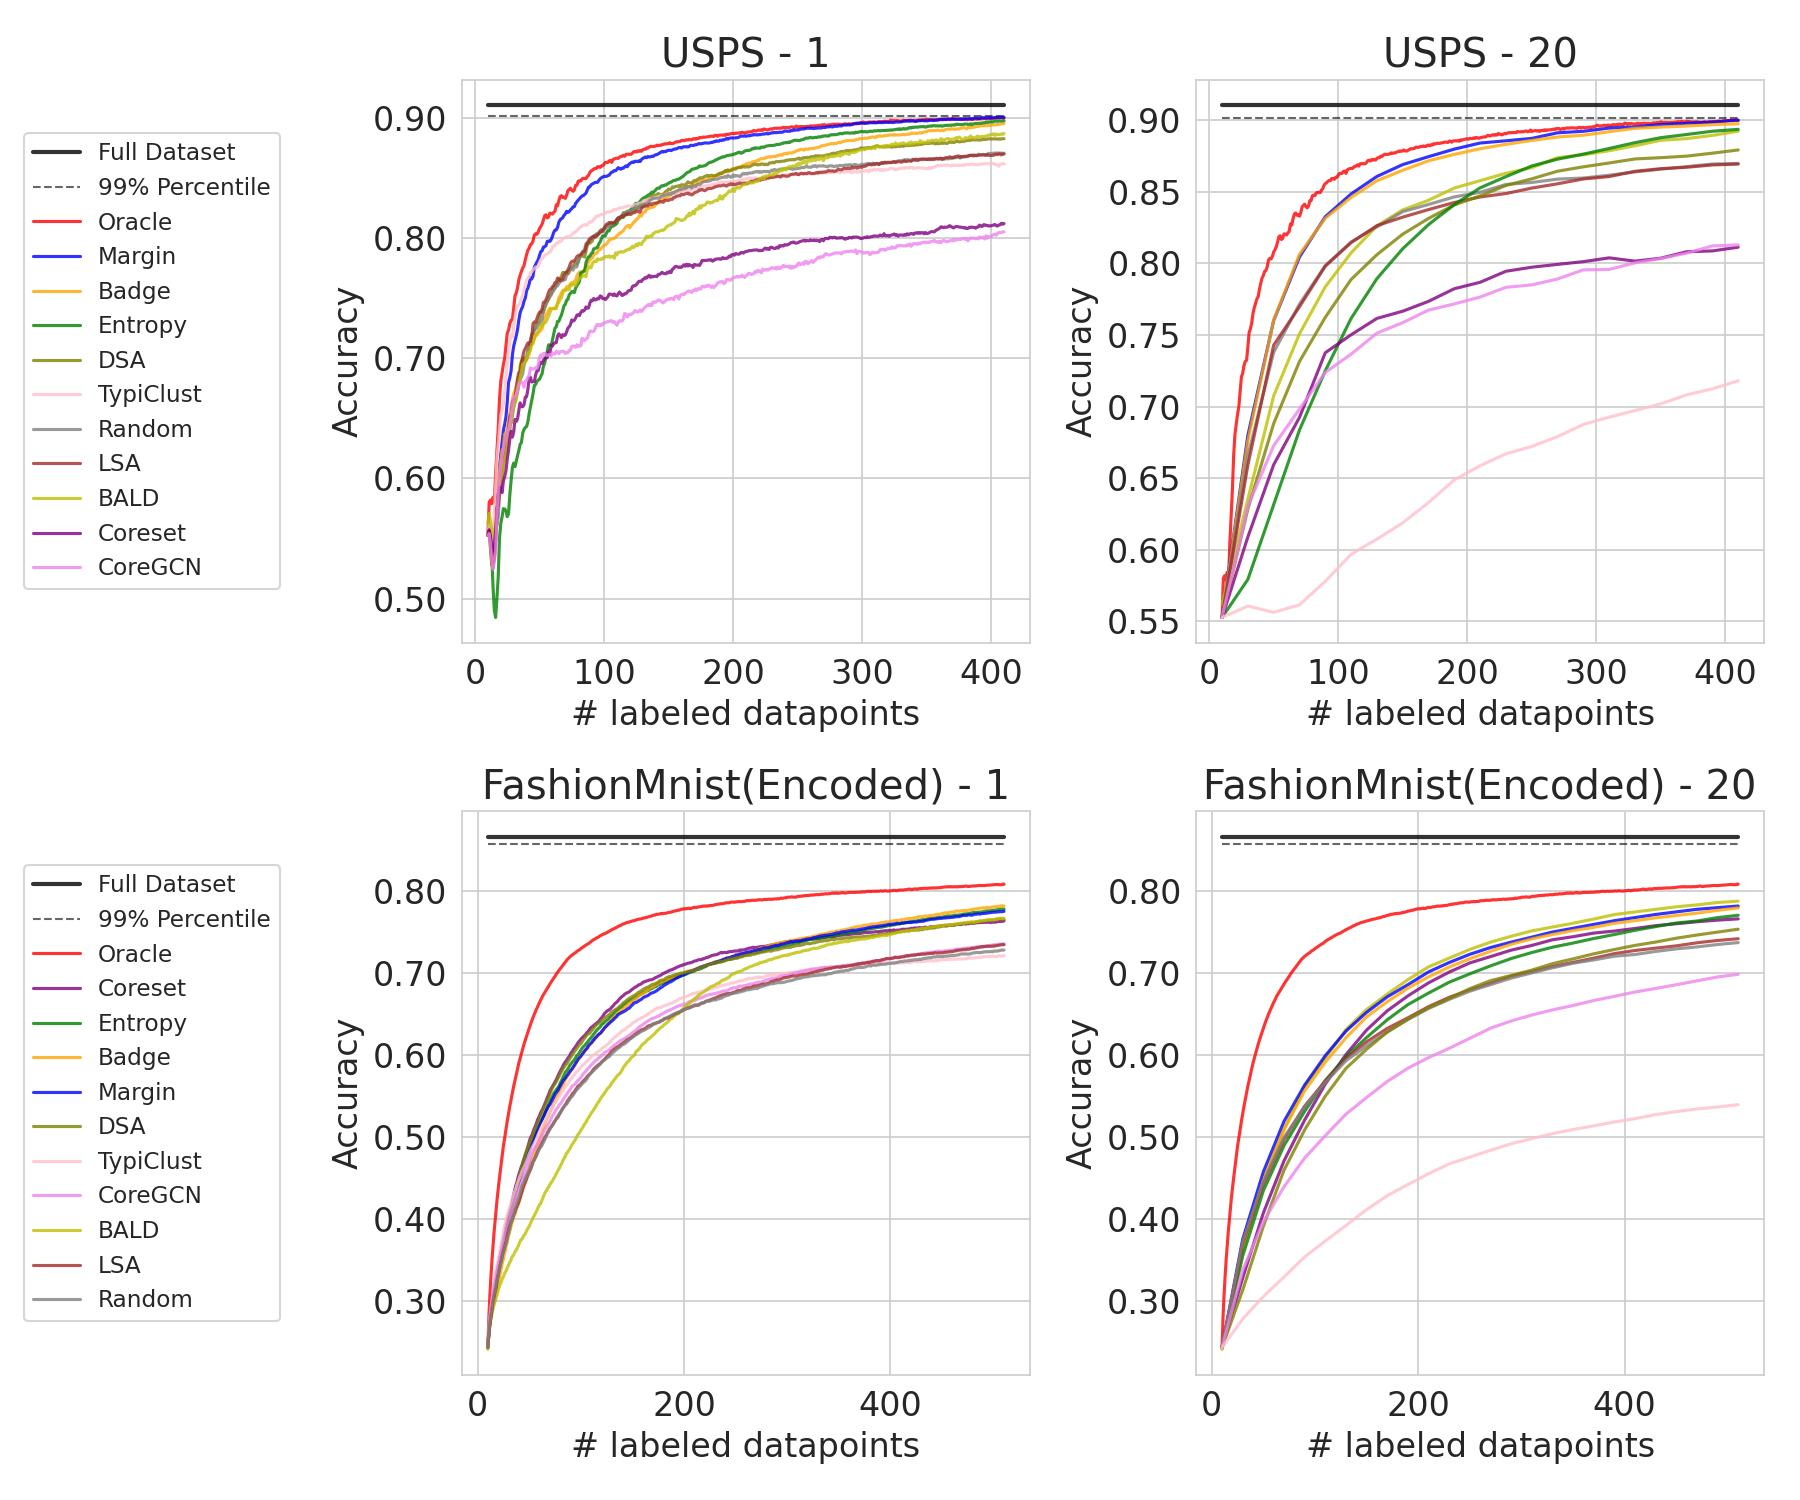
\includegraphics[width=0.9\linewidth]{img/main_body_result.jpg}
%\end{figure}
%
\begin{figure}
    \centering
    \caption{Ranks of each acquisition function aggregated by domain.}
    \label{fig:ranks_by_domain}
    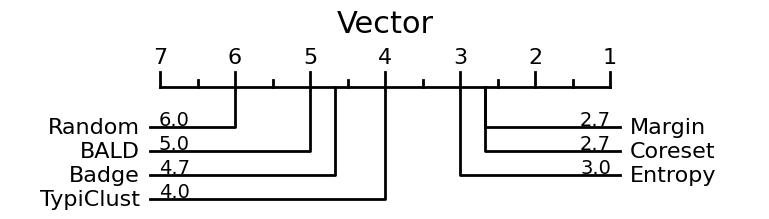
\includegraphics[width=0.49\linewidth]{img/macro_vector.jpg}
    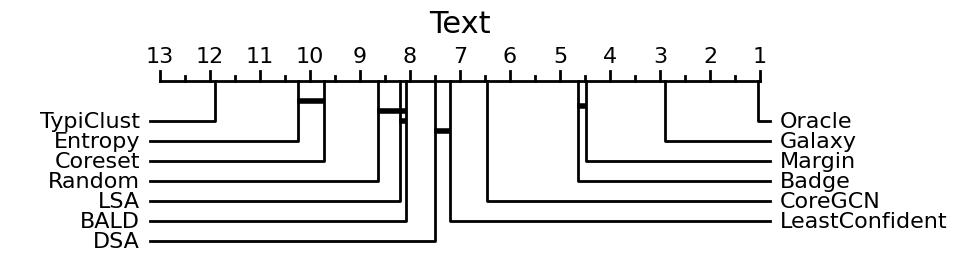
\includegraphics[width=0.49\linewidth]{img/macro_text.jpg}
    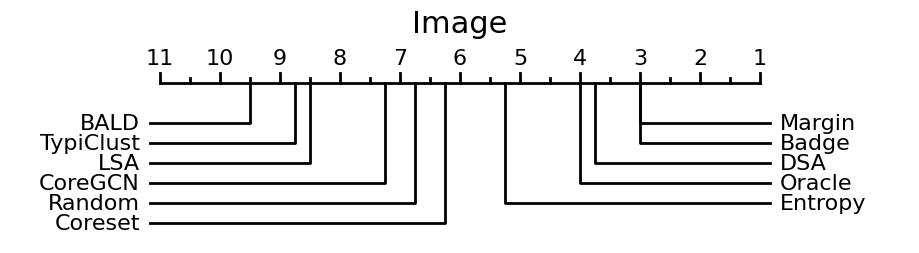
\includegraphics[width=0.49\linewidth]{img/macro_img.jpg}
    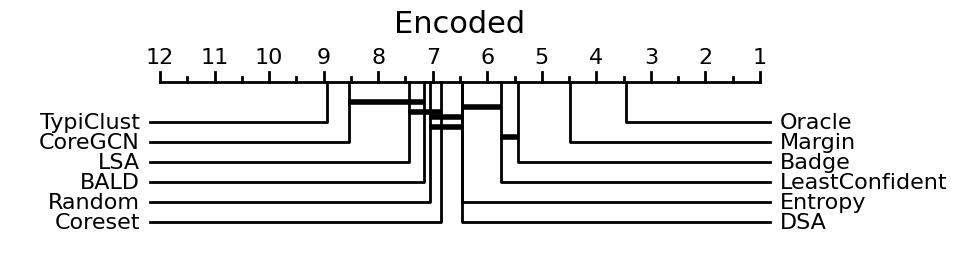
\includegraphics[width=0.49\linewidth]{img/macro_enc.jpg}
\end{figure}
%
\begin{figure}
    \centering
    \caption{Results for all acquisition functions on both synthetic datasets.}
    \label{fig:main_body_result}
    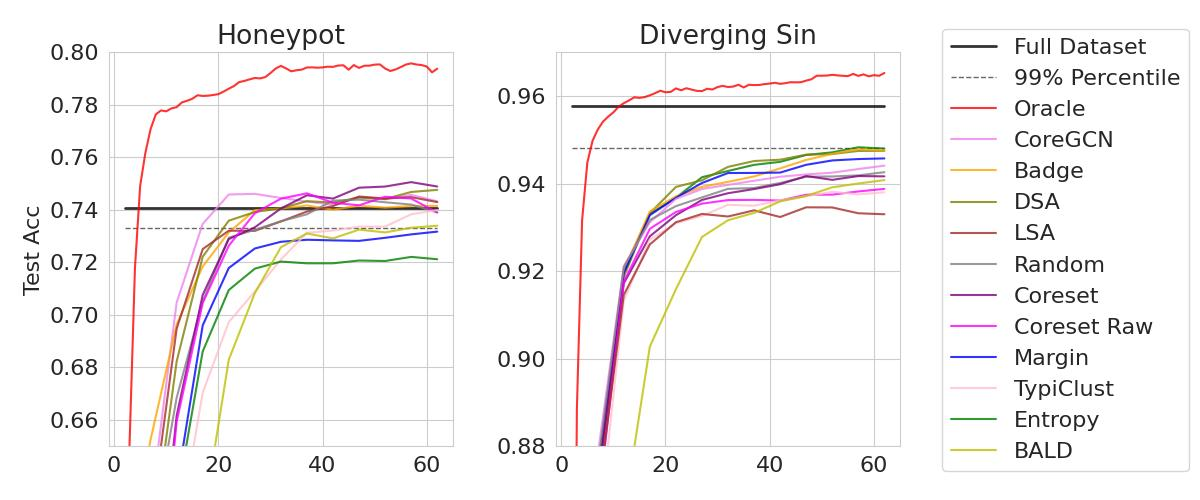
\includegraphics[width=0.9\linewidth]{img/synth_trajectories.jpg}
\end{figure}
Storing the results of every run in a separate file allows us to create various aggregates.
Apart from plotting standard performance curves and reporting their AUC values per dataset (Fig. \ref{fig:main_body_result}), we primarily rely on ranks to aggregate the performance of an acquisition function across datasets.
For each dataset, the AUC values of all acquisition functions are sorted and assigned a rank based on position, with the best rank being 1.
These ranks can safely be averages across datasets as they are no longer subjected to scaling differences of each dataset.
In Table \ref{tab:results} we provide the rank of each acquisition function per dataset and averaged for each (un-)encoded dataset. \\
Additionally, we provide aggregated ranks per data domain in Fig. \ref{fig:ranks_by_domain}, revealing varying performances of acquisition functions like DSA/LSA, BALD and CoreGCN.
The leading algorithms Margin-Sampling and BADGE show very stable performance across all tested data domains. \\ [1mm]
Results for the Honeypot dataset reveal expected shortcomings of uncertainty sampling algorithms like margin and entropy sampling, but also show that BADGE is underperforming for this dataset. 
This is an important result, as margin sampling and BADGE were evaluated to be the best performing acquisition functions for real-world data.
Both being highly vulnerable to adverse samples or simply measurement noise highlights the need for further research in this area. \\
Results for Diverging Sine also confirm expected behaviour, as clustering algorithms (Coreset, TypiClust) fall behind uncertainty algorithms (Entropy-, Margin-Sampling), with the exception of BADGE.
The fact that BADGE is able to perform well on this dataset highlights the importance of embeddings in the clustering algorithms, as the so-called gradient embedding from BADGE seems to be able to encode uncertainty information, guiding the selection into the left hand regions of the dataset.
We provide additional evidence for the importance of the embeddings by testing a version of Coreset on this dataset that does not use the embeddings produced by the classification model, but rather clusters the data directly.
This "Coreset Raw" algorithm performs notably worse than its embedding-based counterpart. \\
We strongly advocate to test newly proposed AL algorithms not only on our benchmark suite of real data, but also pay close attention to Honeypot and Diverging Sine to reveal principled shortcomings of the algorithm.

\newpage
\paragraph{Acknowledgement}
anonymous
%TODO
%Funded by the Lower Saxony Ministry of Science and Culture under grant number ZN3492 within the Lower Saxony “Vorab“ of the Volkswagen Foundation and supported by the Center for Digital Innovations (ZDIN).



\bibliographystyle{plain}
\bibliography{al_benchmark_paper.bib} 

\appendix
\newpage

\section{Problem Formulation}\label{app:problem_formulation}
Given
\begin{itemize}
	\item a number $B\in\N$ (called budget),
	\item two spaces $\X$ and $\Y$,  {\tiny e.g., $\X:=\R^M, \Y:=\R^T$},
	\item a sample $\D_1,\ldots,\D_N \in (\X\times \Y)^*$ of
	sequences of pairs $(x,y)$  from an unknown distribution $p$
	(called datasets),
	%  {\tiny with $|\D_n|\geq B$ for all $n\in 1{:}N$,}
	{\tiny with $p(\D)=0$ for $|\D|<B$,}
	\item a function $\ell:\Y\times\Y\rightarrow\R$ (called loss), and
	\item a function $\hat y:  (\X\times \Y)^* \times \X^* \rightarrow \Y^\X$
	(called learning algorithm), \\
	{\tiny where $\Y^\X$ is the space of all function from $\X$ to $\Y$}
\end{itemize}
find a function
\vspace*{-0.5cm}
\begin{align*}
	\Omega: (\X\times \Y)^* \times \X^* &\rightarrow \N
	\quad\quad \text{\tiny (with $a(\D,X) \leq |X|$)} \\
	& \text{\tiny where $a(\D,X)$ selects an unlabeled instance from $X$}
\end{align*}
% which is equivariant in the second argument,

called acquisition function,
s.t. the expected loss of a model learned on all predictors plus $B$ sequentially acquired targets
is minimal:
\begin{align*}
	\min\ \EE\   &  \{
	% \operatorname{avg}\limits_{(x,y)\in\D\test} \ell(y, \hat y(x))
	\ell(\hat y, \D\test)
	\mid \D\sim p, (\D\train,\D\test):= \text{split}(\D) \}
	\\
	\text{with }
	\hat y:= & A( (\D_{\train_{n_1}},\ldots,\D_{\train_{n_B}}), \D\train|_{\X})
	\\ 
	n_b := & a( (\D_{\train_{n_1}},\ldots,\D_{\train_{n_{b-1}}}), \D\train|_{\X}) ,
	\quad b\in 1{:}B
\end{align*}


%%%%%%%%%%%%%%%%%%%%%%%%%%%%%%%%%%%%%%%%%%%%%%%%%%%%%%%%%%%
%%%%%%%%%%%%%%%%%%%%%%%%%%%%%%%%%%%%%%%%%%%%%%%%%%%%%%%%%%%
\section{Acquistion Functions}\label{app:acquisition_functions}
\textbf{Uncertainty Sampling} 
tries to find the sample that the classifier is most uncertain about by computing heuristics of the class probabilities. For our benchmark, we use entropy and margin (a.k.a. best-vs-second-best) sampling.\\
\textbf{BALD \cite{kirsch2019batchbald}}
applies the query-by-committee strategy of model ensembles to a single model by interpreting the classifier's parameters as distributions and then sample multiple outputs from them via Monte-Carlo dropout.\\
\textbf{BADGE \cite{ashdeep}} uses gradient embeddings of unlabeled points to select samples where the classifier is expected to change a lot. The higher the magnitude of the gradient the higher the expected improvement in model performance.\\
\textbf{Coreset \cite{sener2017active}}
employs K-Means clustering trying to cover the whole data distribution.
Selects the unlabeled sample that is the furthest away from all cluster centers.
Clustering is done in a semantically meaningful space by encoding the data with the current classifier $\hat y$.
In this work, we use the greedy variant of Coreset.\\
\textbf{TypiClust \cite{hacohen2022active}}
relies on clustering similar to Coreset, but proposes a new measure called ``Typicality" to select unlabeled samples.
It selects points that are in the densest regions of clusters that do not contain labeled samples yet.
Clustering is done in a semantically meaningful space by encoding the data with the current classifier $\hat y$.
It has to be pointed out that TypiClust was designed for low-budget scenarios, but we think it is still worthwhile to test and compare this algorithm with higher budgets. \\
\textbf{Core-GCN \cite{caramalau2021sequential}} TODO \\
\textbf{DSA/LSA \cite{kim2019guiding}} TODO \\ [2mm]
%
\textbf{Excluded Algorithms}\\
\textbf{Learning Loss for AL \cite{yoo2019learning}}
Introduces an updated training of the classification model with an auxiliary loss and therefore cannot be compared fairly against classification models without this boosted training regime.\\ [1mm]
%
\textbf{Reinforcement Learning Algorithms} \\
TODO \\


%%%%%%%%%%%%%%%%%%%%%%%%%%%%%%%%%%%%%%%%%%%%%%%%%%%%%%%%%
%%%%%%%%%%%%%%%%%%%%%%%%%%%%%%%%%%%%%%%%%%%%%%%%%%%%%%%%%
\section{All Results}\label{app:all_results}
% Splice
\begin{minipage}{0.65\linewidth}
\begin{figure}[H]
    \centering
    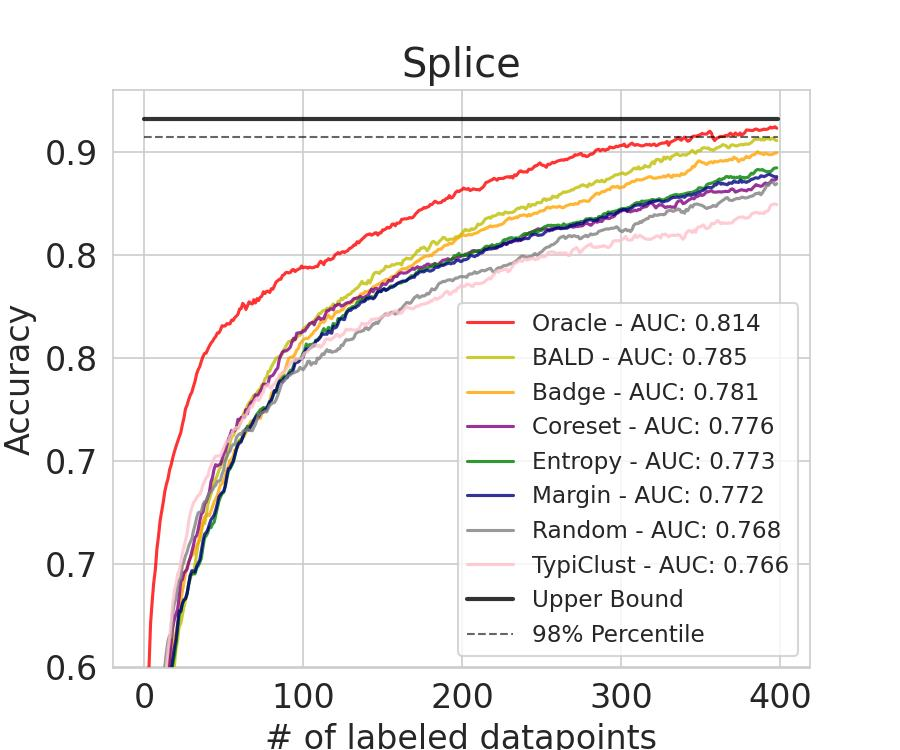
\includegraphics[width=\linewidth]{img/eval_splice}\\ [2mm]
    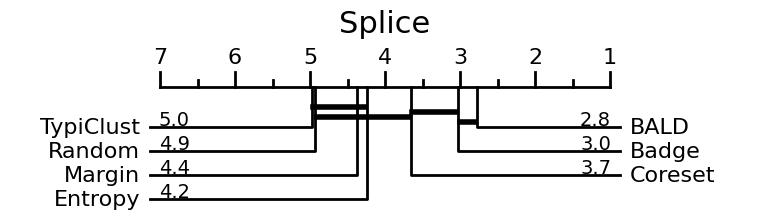
\includegraphics[width=\linewidth]{img/micro_splice.jpg}
\end{figure}
\end{minipage}
\begin{minipage}{0.29\linewidth}
\begin{tabular}{c|c}
    &Splice \\
    \hline
    Oracle&0.811 $\pm$ 0.010\\
    BALD&0.785 $\pm$ 0.013\\
    Coreset&0.778 $\pm$ 0.014\\
    Entropy&0.774 $\pm$ 0.016\\
    Margin&0.773 $\pm$ 0.016\\
    Badge&0.770 $\pm$ 0.016\\
    Random&0.768 $\pm$ 0.014\\
    TypiClust&0.766 $\pm$ 0.014\\
\end{tabular}
\end{minipage}
%DNA
\begin{minipage}{0.65\linewidth}
\begin{figure}[H]
    \centering
	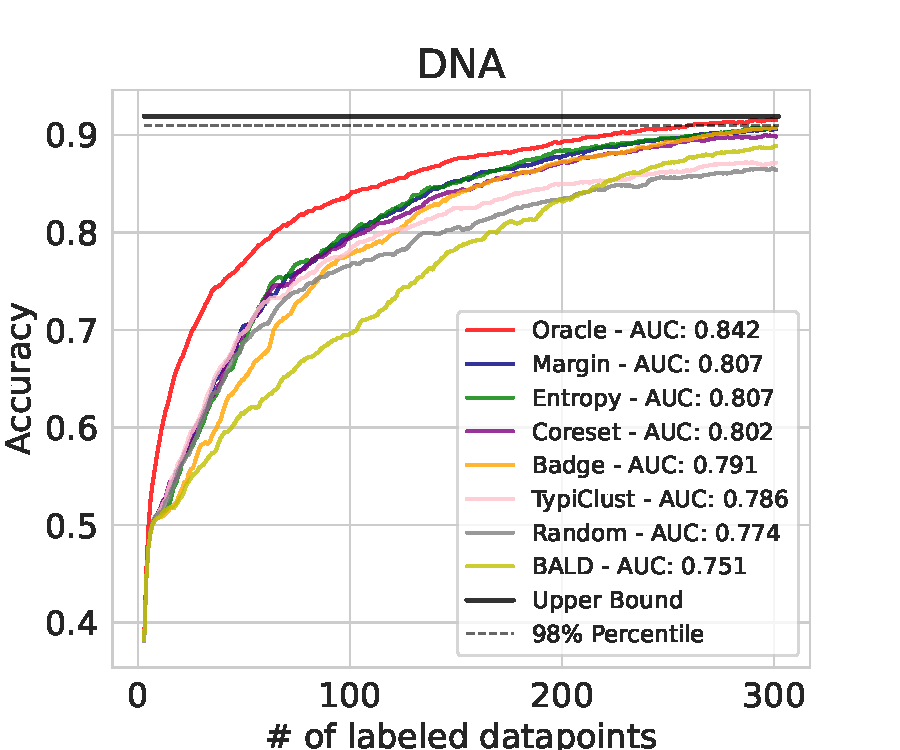
\includegraphics[width=\linewidth]{img/eval_dna} \\ [2mm]
        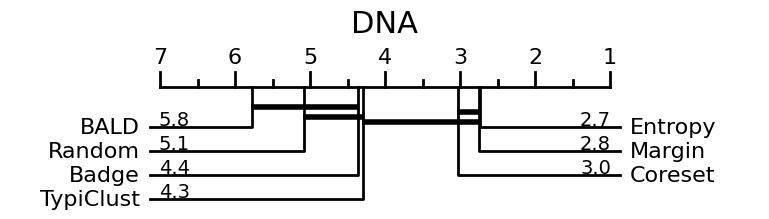
\includegraphics[width=\linewidth]{img/micro_dna.jpg}
\end{figure}
\end{minipage}
\begin{minipage}{0.29\linewidth}
\begin{tabular}{c|c}
&DNA \\
\hline
Oracle&0.842 $\pm$ 0.021\\
Margin&0.807 $\pm$ 0.035\\
Entropy&0.805 $\pm$ 0.038\\
Coreset&0.796 $\pm$ 0.028\\
Badge&0.789 $\pm$ 0.056\\
TypiClust&0.788 $\pm$ 0.036\\
Random&0.768 $\pm$ 0.024\\
BALD&0.749 $\pm$ 0.044\\
\end{tabular}
\end{minipage}
%USPS
\begin{minipage}{0.65\linewidth}
\begin{figure}[H]
    \centering
	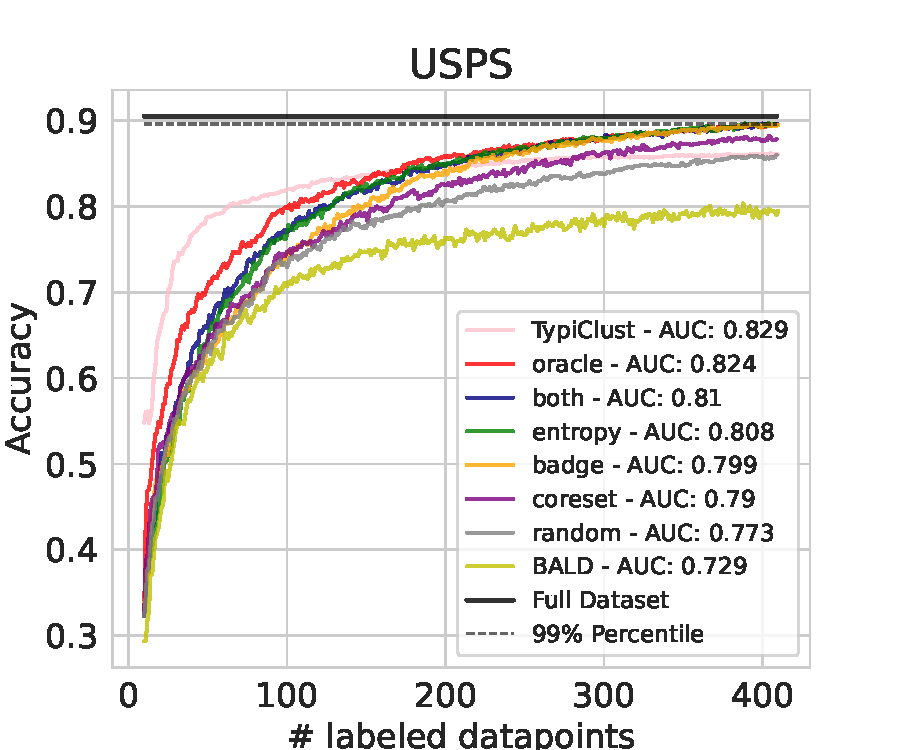
\includegraphics[width=\linewidth]{img/eval_usps} \\ [2mm]
	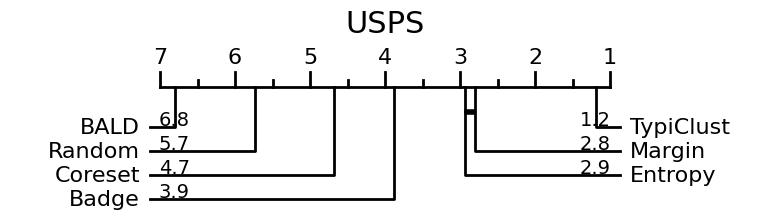
\includegraphics[width=\linewidth]{img/micro_usps.jpg}
\end{figure}
\end{minipage}
\begin{minipage}{0.29\linewidth}
\begin{tabular}{c|c}
&USPS\\
\hline
TypiClust&0.830 $\pm$ 0.007\\
Oracle&0.823 $\pm$ 0.011\\
Margin&0.809 $\pm$ 0.013\\
Entropy&0.807 $\pm$ 0.013\\
Badge&0.795 $\pm$ 0.018\\
Coreset&0.788 $\pm$ 0.017\\
Random&0.774 $\pm$ 0.012\\
BALD&0.725 $\pm$ 0.050\\
\end{tabular}
\end{minipage}
%Splice Enc
\begin{minipage}{0.65\linewidth}
\begin{figure}[H]
    \centering
    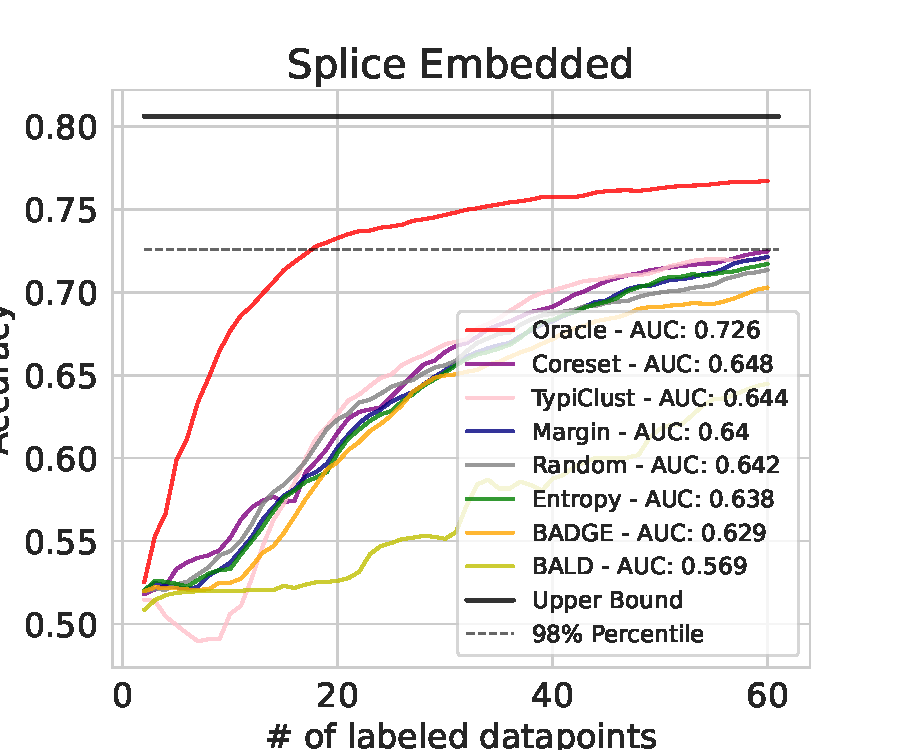
\includegraphics[width=\linewidth]{img/eval_splice_enc} \\ [2mm]
    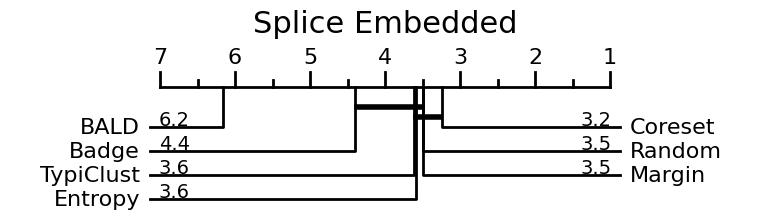
\includegraphics[width=\linewidth]{img/micro_splice_enc.jpg}
\end{figure}
\end{minipage}
\begin{minipage}{0.29\linewidth}
\begin{tabular}{c|c}
&SpliceEncoded \\
\hline
Oracle&0.728 $\pm$ 0.022\\
Coreset&0.648 $\pm$ 0.027\\
TypiClust&0.645 $\pm$ 0.042\\
Random&0.643 $\pm$ 0.036\\
Entropy&0.636 $\pm$ 0.033\\
Margin&0.636 $\pm$ 0.033\\
Badge&0.627 $\pm$ 0.040\\
BALD&0.565 $\pm$ 0.049\\
\end{tabular}
\end{minipage}
%DNA Enc
\begin{minipage}{0.65\linewidth}
\begin{figure}[H]
    \centering
    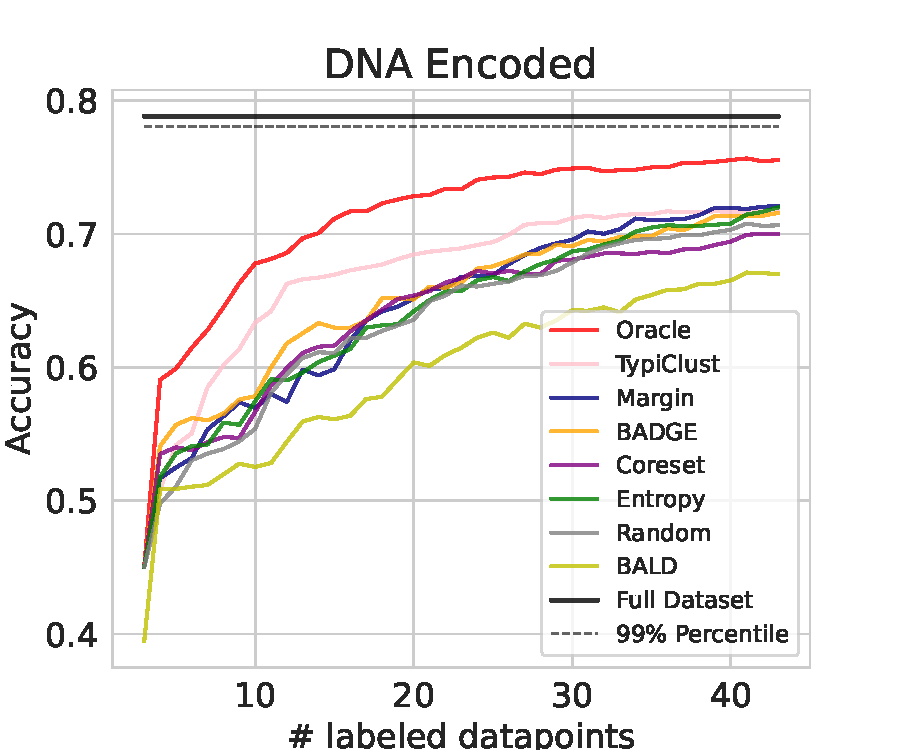
\includegraphics[width=\linewidth]{img/eval_dna_enc}\\ [2mm]
    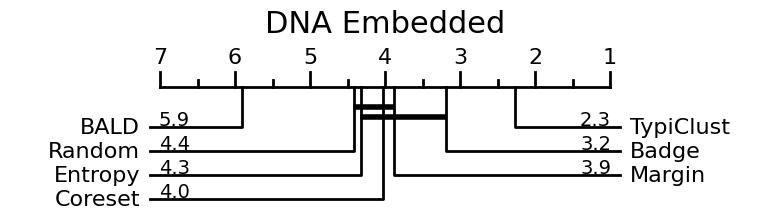
\includegraphics[width=\linewidth]{img/micro_dna_enc.jpg} 
\end{figure}
\end{minipage}
\begin{minipage}{0.29\linewidth}
\begin{tabular}{c|c}
&DNAEncoded\\
\hline
Oracle&0.709 $\pm$ 0.023\\
TypiClust&0.672 $\pm$ 0.029\\
Margin&0.648 $\pm$ 0.047\\
Badge&0.647 $\pm$ 0.037\\
Coreset&0.640 $\pm$ 0.041\\
Entropy&0.629 $\pm$ 0.062\\
Random&0.626 $\pm$ 0.035\\
BALD&0.594 $\pm$ 0.039\\
\end{tabular}
\end{minipage}
%USPS Enc
\begin{minipage}{0.65\linewidth}
\begin{figure}[H]
    \centering
    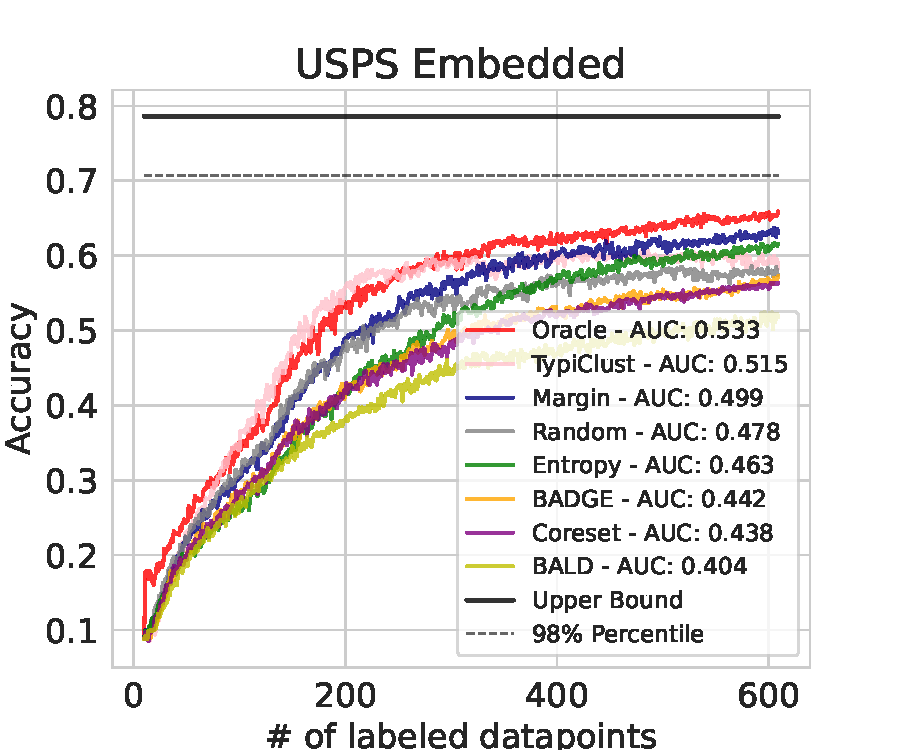
\includegraphics[width=\linewidth]{img/eval_usps_enc}\\ [2mm]
    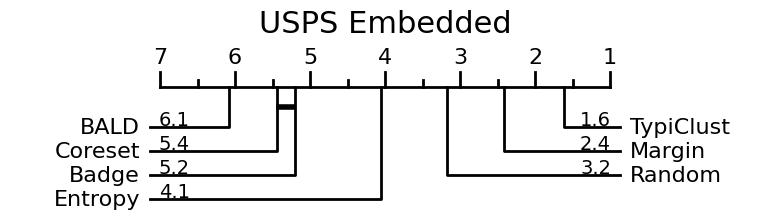
\includegraphics[width=\linewidth]{img/micro_usps_enc.jpg} 
\end{figure}
\end{minipage}
\begin{minipage}{0.29\linewidth}
\begin{tabular}{c|c}
&USPSEncoded\\
\hline
Oracle&0.522 $\pm$ 0.021\\
TypiClust&0.507 $\pm$ 0.025\\
Margin&0.496 $\pm$ 0.030\\
Random&0.468 $\pm$ 0.025\\
Entropy&0.459 $\pm$ 0.021\\
Badge&0.440 $\pm$ 0.026\\
Coreset&0.435 $\pm$ 0.027\\
BALD&0.402 $\pm$ 0.052\\
\end{tabular}
\end{minipage}
%Cifar10
\begin{minipage}{0.65\linewidth}
\begin{figure}[H]
    \centering
    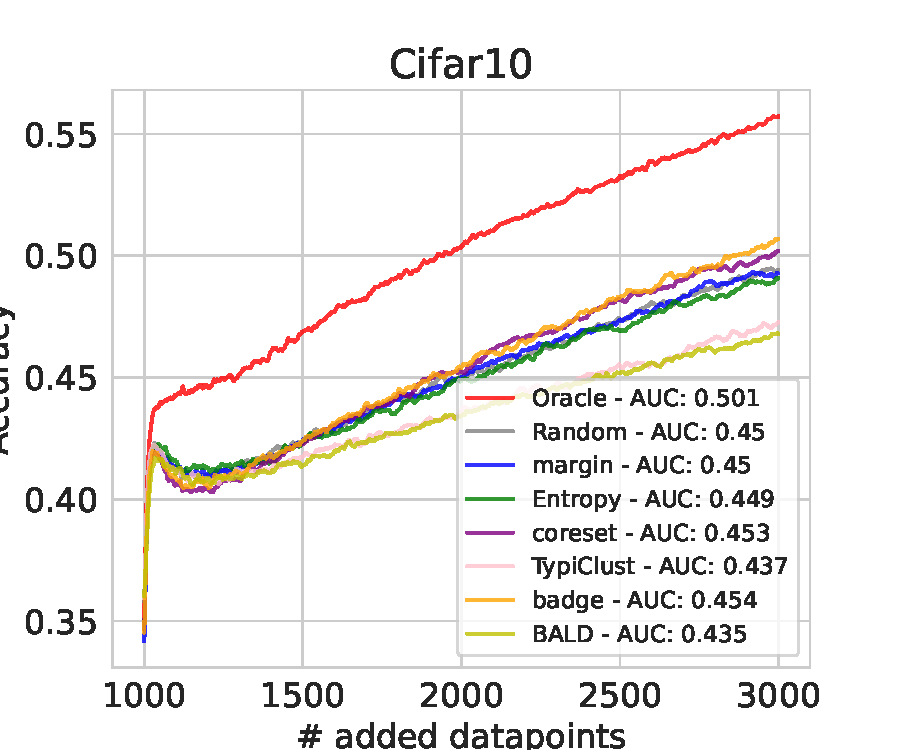
\includegraphics[width=\linewidth]{img/eval_cifar10}\\ [2mm]
    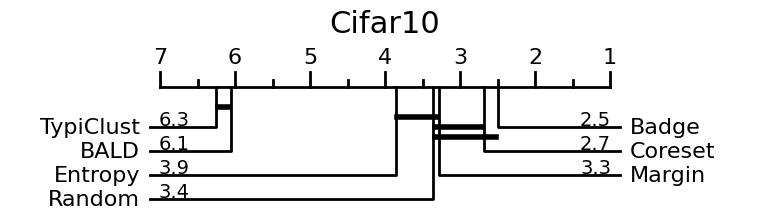
\includegraphics[width=\linewidth]{img/micro_cifar10.jpg}
\end{figure}
\end{minipage}
\begin{minipage}{0.29\linewidth}
\begin{tabular}{c|c}
&Cifar10\\
\hline
Oracle&0.500 $\pm$ 0.010\\
Badge&0.453 $\pm$ 0.012\\
Coreset&0.453 $\pm$ 0.009\\
Margin&0.451 $\pm$ 0.010\\
Random&0.450 $\pm$ 0.012\\
Entropy&0.449 $\pm$ 0.010\\
TypiClust&0.436 $\pm$ 0.010\\
BALD&0.436 $\pm$ 0.010\\
\end{tabular}
\end{minipage}
%FMnist
\begin{minipage}{0.65\linewidth}
\begin{figure}[H]
    \centering
    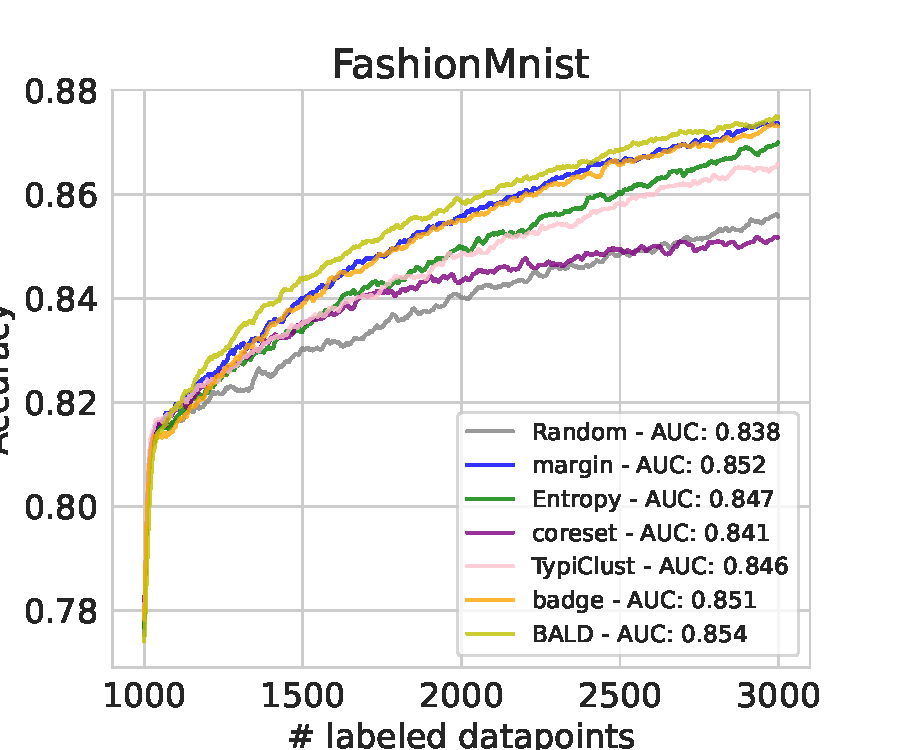
\includegraphics[width=\linewidth]{img/eval_fmnist}\\ [2mm]
    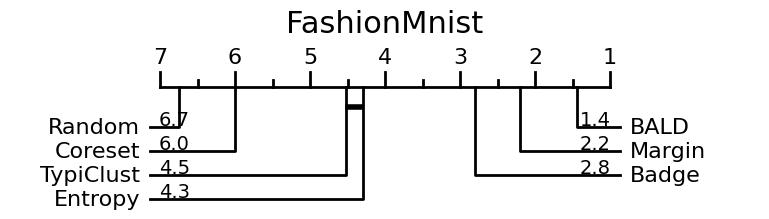
\includegraphics[width=\linewidth]{img/micro_fmnist.jpg}
\end{figure}
\end{minipage}
\begin{minipage}{0.29\linewidth}
\begin{tabular}{c|c}
&FashionMnist\\
\hline
Oracle&0.862 $\pm$ 0.003\\
BALD&0.854 $\pm$ 0.003\\
Margin&0.851 $\pm$ 0.003\\
Badge&0.851 $\pm$ 0.003\\
Entropy&0.847 $\pm$ 0.004\\
TypiClust&0.846 $\pm$ 0.004\\
Coreset&0.840 $\pm$ 0.004\\
Random&0.837 $\pm$ 0.004\\
\end{tabular}
\end{minipage}
%Cifar10 Encoded
\begin{minipage}{0.65\linewidth}
\begin{figure}[H]
    \centering
    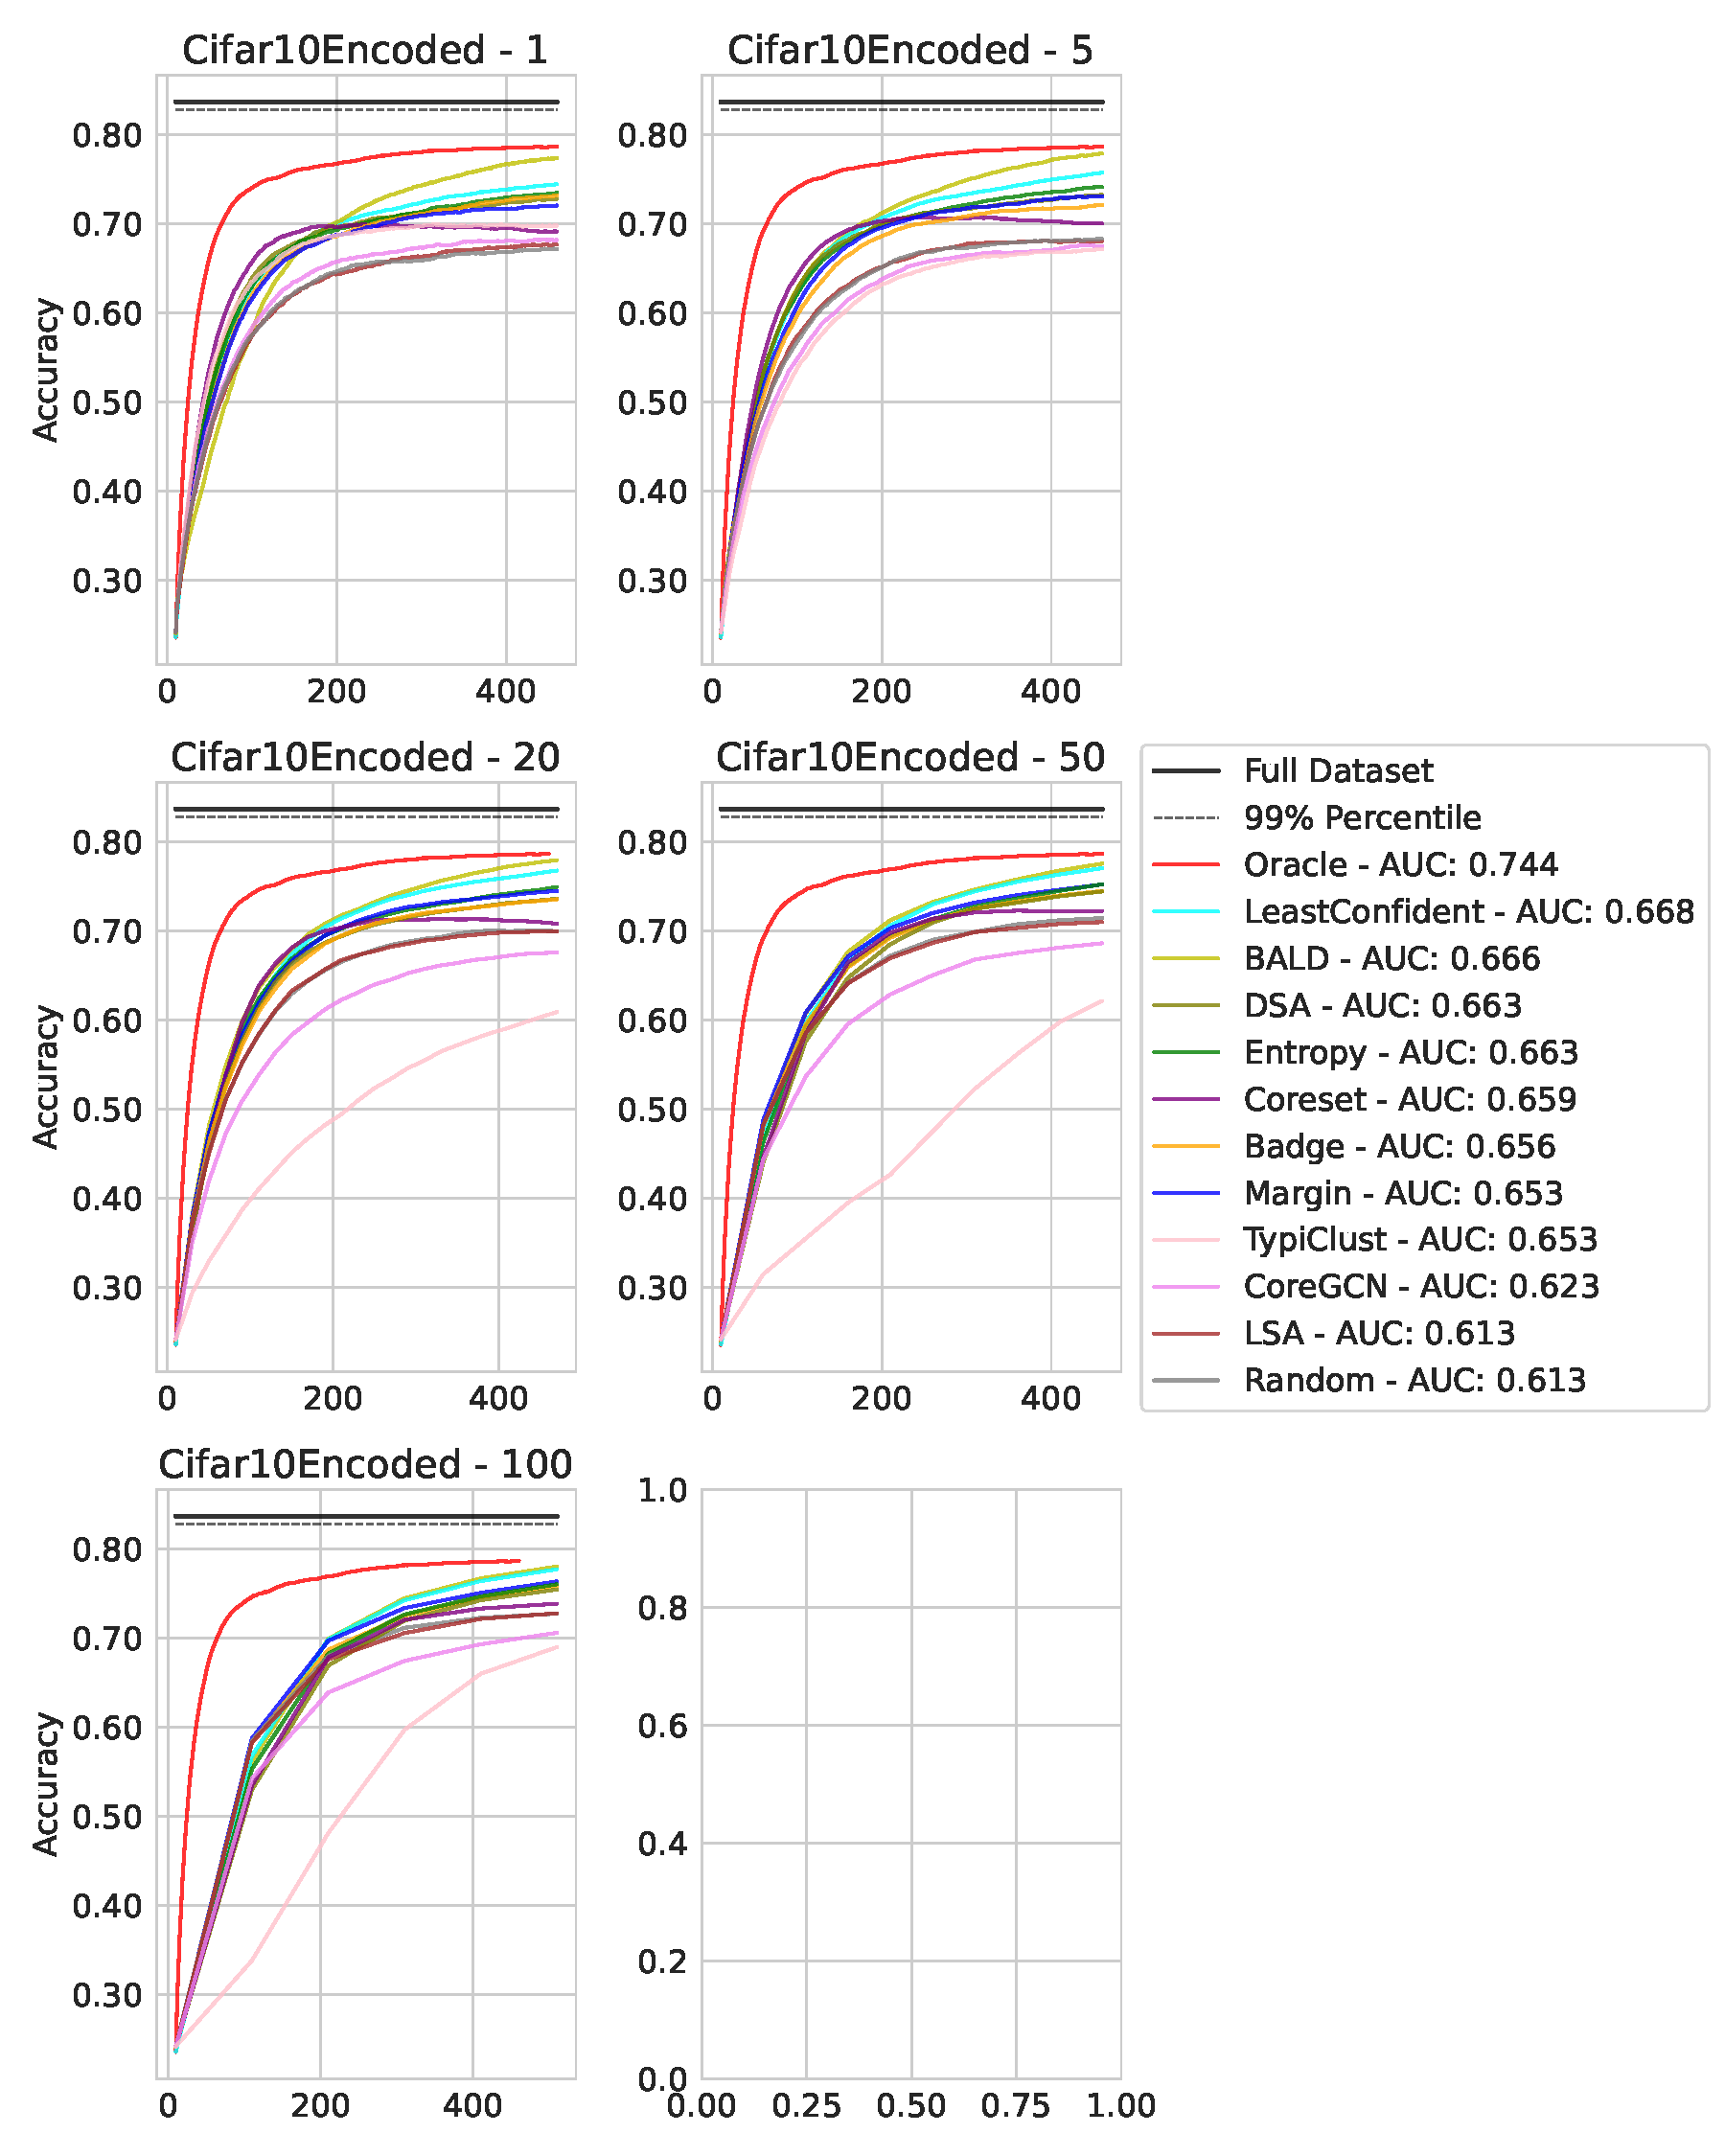
\includegraphics[width=\linewidth]{img/eval_cifar10_enc} \\ [2mm]
    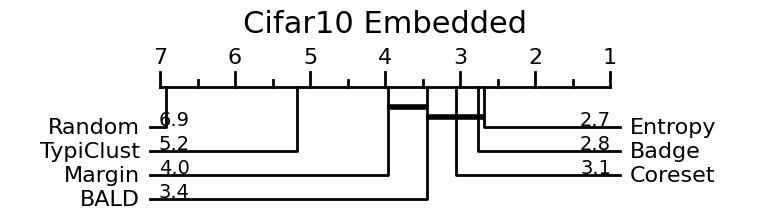
\includegraphics[width=\linewidth]{img/micro_cifar10_enc.jpg} 
\end{figure}
\end{minipage}
\begin{minipage}{0.29\linewidth}
\begin{tabular}{c|c}
&Cifar10Encoded\\
\hline
Oracle&0.714 $\pm$ 0.007\\
Entropy&0.654 $\pm$ 0.013\\
Coreset&0.653 $\pm$ 0.012\\
Badge&0.653 $\pm$ 0.012\\
BALD&0.650 $\pm$ 0.016\\
Margin&0.647 $\pm$ 0.012\\
TypiClust&0.636 $\pm$ 0.009\\
Random&0.607 $\pm$ 0.013\\
\end{tabular}
\end{minipage}
%FashionMnist Encoded
\begin{minipage}{0.65\linewidth}
\begin{figure}[H]
    \centering
    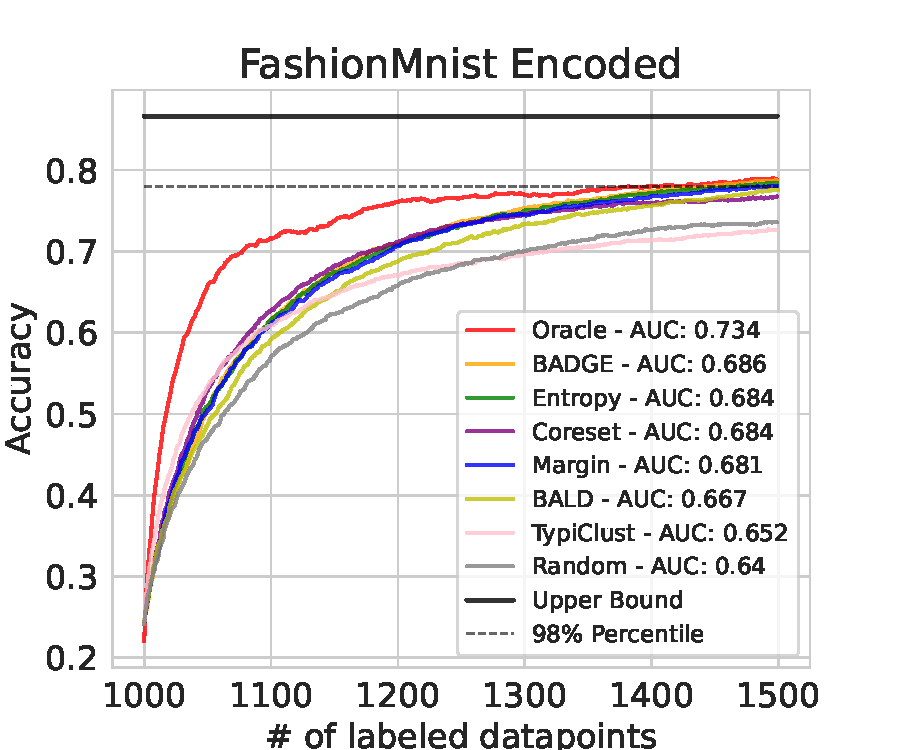
\includegraphics[width=\linewidth]{img/eval_fmnist_enc} \\ [2mm]
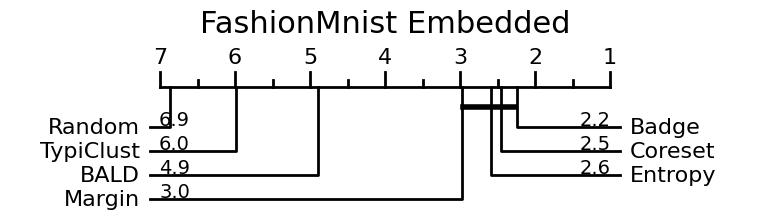
\includegraphics[width=\linewidth]{img/micro_fmnist_enc.jpg} 
\end{figure}
\end{minipage}
\begin{minipage}{0.29\linewidth}
\begin{tabular}{c|c}
&FashionMnistEncoded\\
\hline
Oracle&0.732 $\pm$ 0.006\\
Coreset&0.686 $\pm$ 0.008\\
Badge&0.685 $\pm$ 0.008\\
Entropy&0.684 $\pm$ 0.009\\
Margin&0.682 $\pm$ 0.011\\
BALD&0.668 $\pm$ 0.009\\
TypiClust&0.652 $\pm$ 0.009\\
Random&0.640 $\pm$ 0.011\\
\end{tabular}
\end{minipage}
%TopV2
\begin{minipage}{0.65\linewidth}
\begin{figure}[H]
    \centering
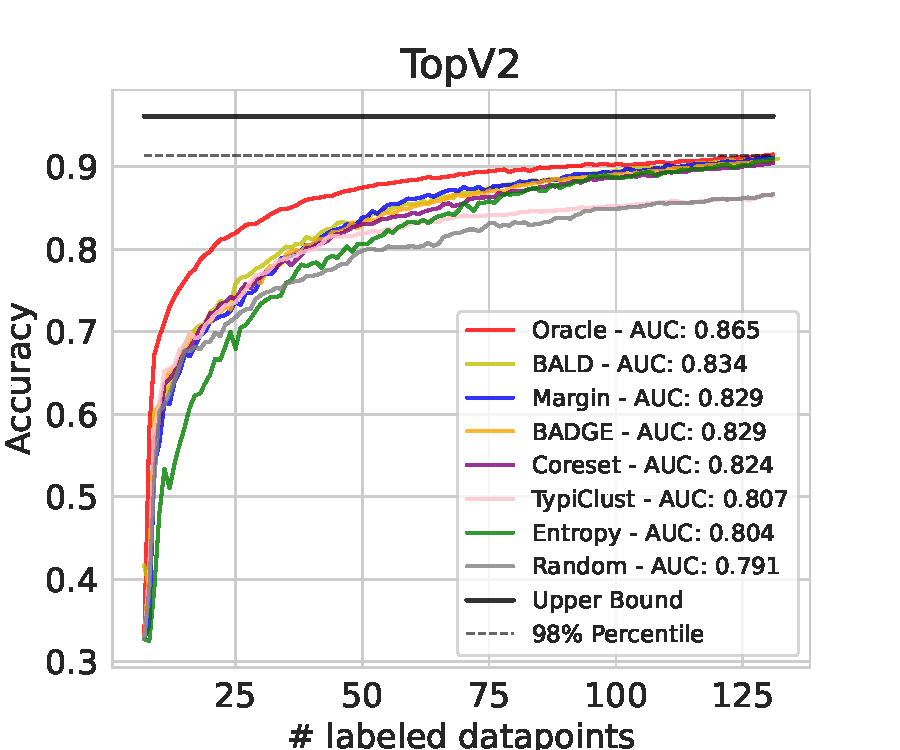
\includegraphics[width=\linewidth]{img/eval_topv2} \\[2mm]
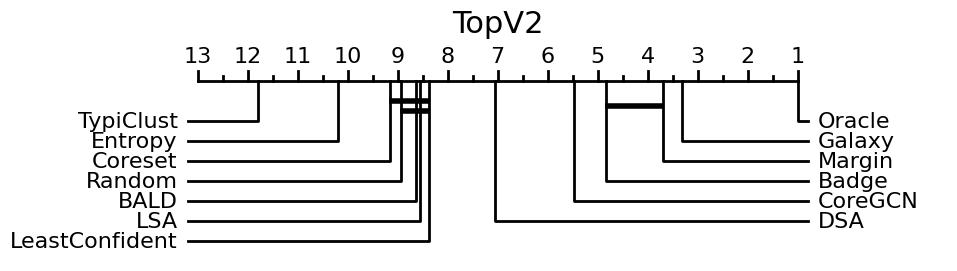
\includegraphics[width=\linewidth]{img/micro_topv2.jpg}
\end{figure}
\end{minipage}
\begin{minipage}{0.29\linewidth}
\begin{tabular}{c|c}
&TopV2\\
\hline
Oracle&0.862 $\pm$ 0.006\\
BALD&0.831 $\pm$ 0.013\\
Badge&0.826 $\pm$ 0.015\\
Coreset&0.823 $\pm$ 0.016\\
Margin&0.822 $\pm$ 0.015\\
TypiClust&0.805 $\pm$ 0.015\\
Entropy&0.801 $\pm$ 0.025\\
Random&0.787 $\pm$ 0.015\\
\end{tabular}
\end{minipage}
%News
\begin{minipage}{0.65\linewidth}
\begin{figure}[H]
    \centering
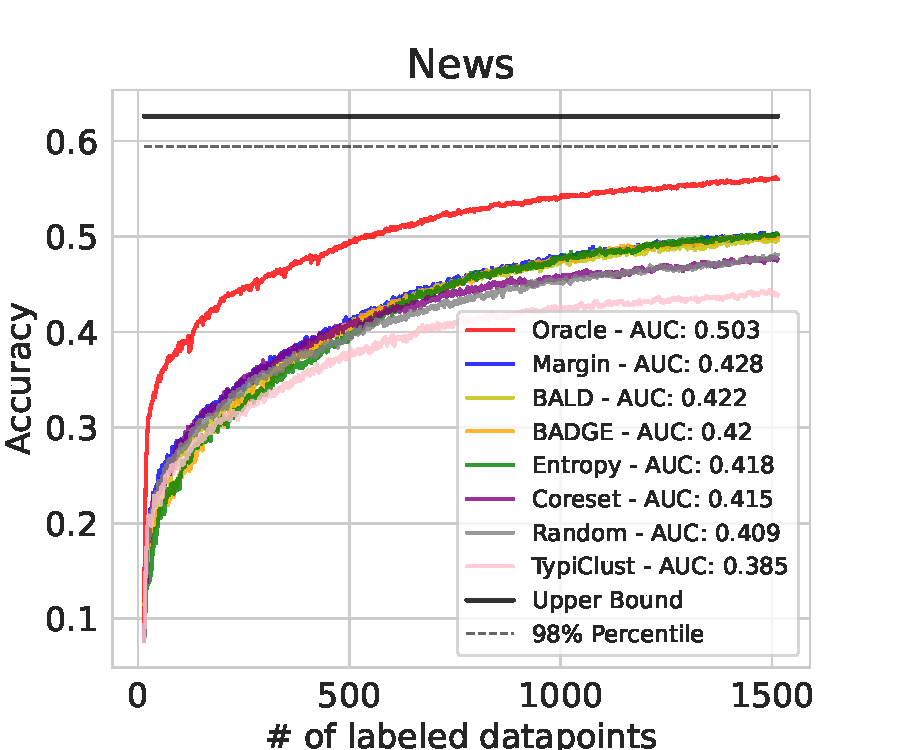
\includegraphics[width=\linewidth]{img/eval_news} \\[2mm]
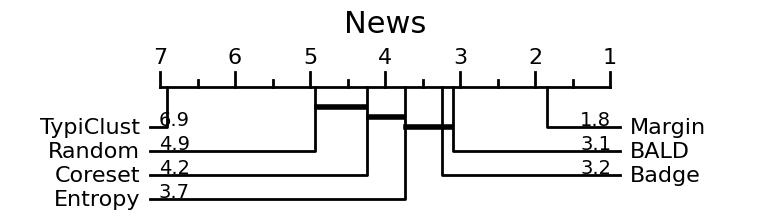
\includegraphics[width=\linewidth]{img/micro_news.jpg}
\end{figure}
\end{minipage}
\begin{minipage}{0.29\linewidth}
\begin{tabular}{c|c}
&News\\
\hline
Oracle&0.502 $\pm$ 0.005\\
Margin&0.427 $\pm$ 0.007\\
BALD&0.421 $\pm$ 0.008\\
Badge&0.420 $\pm$ 0.011\\
Entropy&0.416 $\pm$ 0.010\\
Coreset&0.415 $\pm$ 0.011\\
Random&0.409 $\pm$ 0.008\\
TypiClust&0.385 $\pm$ 0.010\\
\end{tabular}
\end{minipage}
%ThreeClust
\begin{minipage}{0.65\linewidth}
\begin{figure}[H]
    \centering
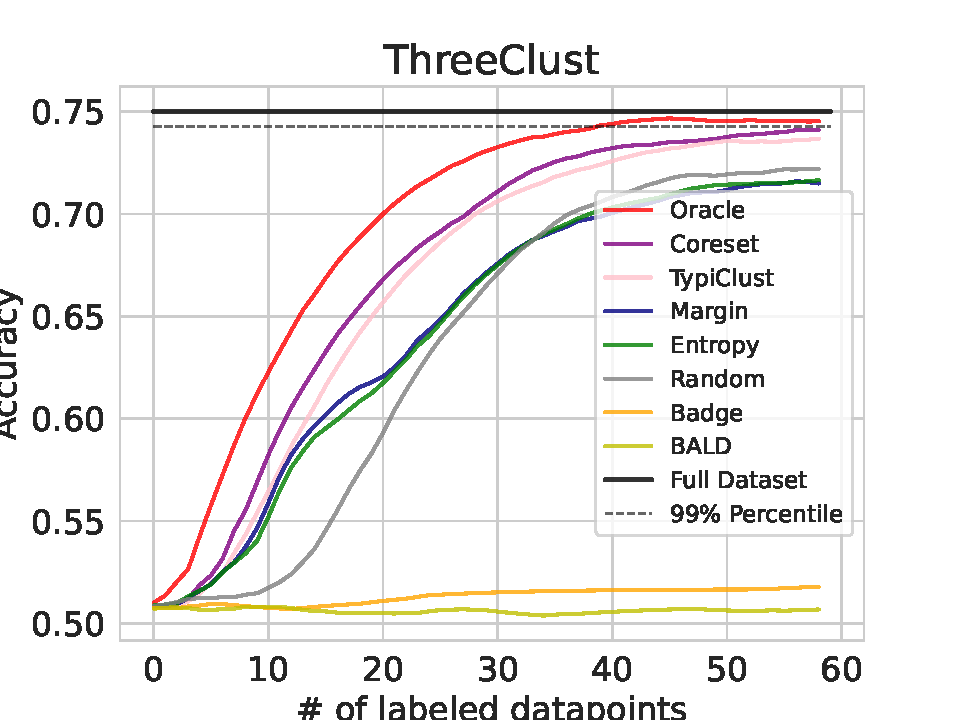
\includegraphics[width=\linewidth]{img/eval_threeclust.pdf} \\[2mm]
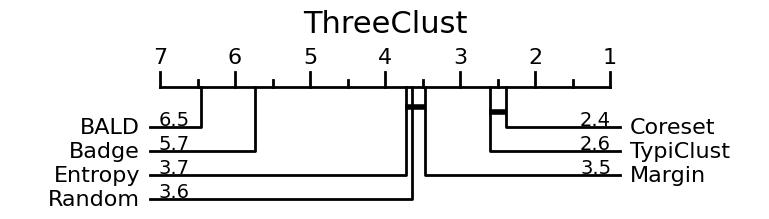
\includegraphics[width=\linewidth]{img/micro_threeclust.jpg}
\end{figure}
\end{minipage}
\begin{minipage}{0.29\linewidth}
\begin{tabular}{c|c}
&ThreeClust \\
\hline
Oracle&0.722 $\pm$ 0.097\\
Coreset&0.698 $\pm$ 0.058\\
TypiClust&0.697 $\pm$ 0.055\\
Entropy&0.682 $\pm$ 0.098\\
Random&0.672 $\pm$ 0.067\\
Margin&0.669 $\pm$ 0.095\\
Badge&0.524 $\pm$ 0.086\\
BALD&0.507 $\pm$ 0.050\\
\end{tabular}
\end{minipage}
%DivergingSin
\begin{minipage}{0.65\linewidth}
\begin{figure}[H]
    \centering
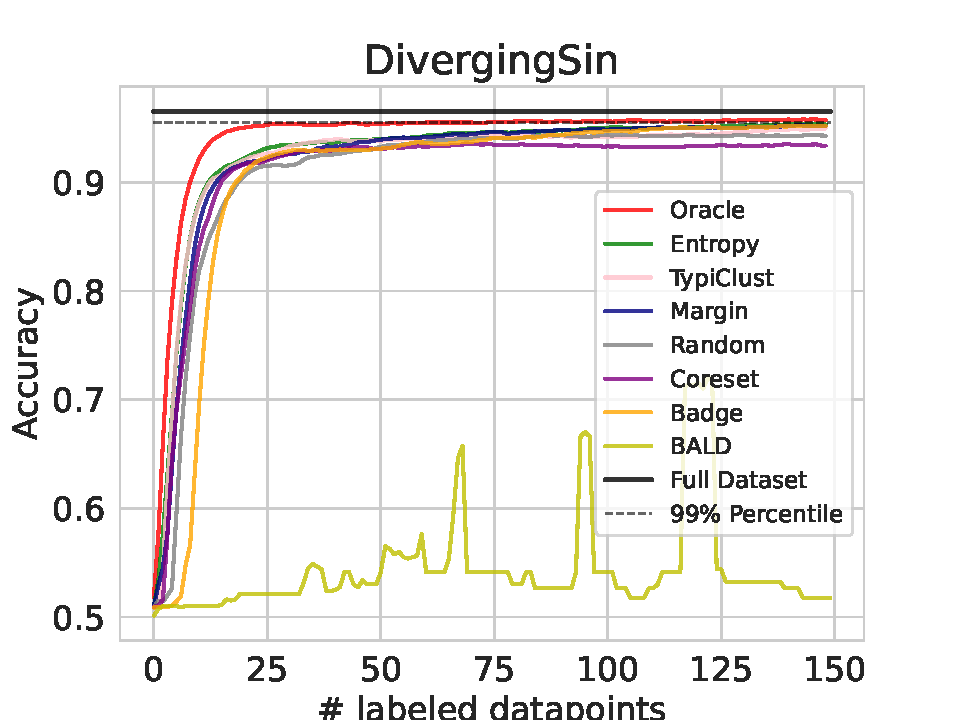
\includegraphics[width=\linewidth]{img/eval_divergingsin.pdf} \\[2mm]
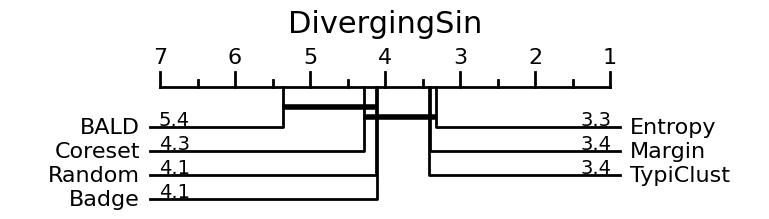
\includegraphics[width=\linewidth]{img/micro_divsin.jpg}
\end{figure}
\end{minipage}
\begin{minipage}{0.29\linewidth}
\begin{tabular}{c|c}
&DivergingSin\\
\hline
Oracle&0.948 $\pm$ 0.198\\
Entropy&0.936 $\pm$ 0.202\\
TypiClust&0.930 $\pm$ 0.196\\
Margin&0.929 $\pm$ 0.201\\
Random&0.919 $\pm$ 0.191\\
Badge&0.914 $\pm$ 0.202\\
Coreset&0.914 $\pm$ 0.197\\
BALD&0.661 $\pm$ 0.167\\
\end{tabular}
\end{minipage}


\section{Seeding Strategy}\label{app:seeding_strategy}
We aim to provide an experimental setup that is fully reproducible independent of the dataset, classification model, or AL algorithm used.
For a fair comparison of two AL algorithms, both algorithms need to receive equal starting conditions in terms of train/validation split, initialization of classifier, and even the state of minor systems like the optimizer or mini-batch sampler.
Even though different implementations might have their own solution to some of these problems, only \cite{ji2023randomness} has described and implemented a fully reproducible pipeline for AL evaluation.
The term reproducibility in this work is used as a synonym not only for the reproducibility of an experiment (a final result given a seed), but also the reproducibility of all subsystems independent of each other.
The seed for one subsystem should always reproduce the behavior of this subsystem independent of all other subsystems and their seeds.
The main obstacle for ensuring reproducibility is the seeding utility in PyTorch, Tensorflow, and other frameworks, whose default choice is a single global seed.
Since many subsystems draw random numbers from this seed, all of them influence each other to a point where a single additional draw can completely change the model initialization, data split or the order of training batches.
Even though some workarounds exist, e.g. re-setting the seed multiple times, this problem is not limited to the initialization phase, but also extends to the AL iterations and the systems within.
We propose an implementation that creates separate Random Number Generators (RNGs) for each of these systems to ensure equal testing conditions even when the AL algorithm, dataset, or classifier changes.
We hypothesize that the insufficient setup with global seeds contributes to the ongoing problem of inconsistent results of AL algorithms in different papers. \\ [1mm]
In summary, we introduce three different seeds: $s_\Omega$ for the AL algorithm, $s_\mathcal{D}$ for dataset splitting and mini-batch sampling, and $s_\theta$ for model initialization and sampling of dropout masks.
Unless stated otherwise, we will keep $s_\Omega$ fixed, while $s_\mathcal{D}$ and $s_\theta$ are incremented by 1 between restarts to introduce stochasticity into our framework.
Some algorithms require a subsample to be drawn from $\mathcal{U}$ in order to reduce the computational cost in each iteration, while others need access to the full unlabeled pool (e.g. for effective clustering).
If a subsample is required, it will be drawn from $s_\Omega$ and therefore will not influence other systems in the experiments.
For each algorithm, we decided if subsampling is required based on our available hardware, but decided against setting a fixed time limit per experiment, since this would introduce unnecessary complexity into the benchmark.
An overview of selected hyperparameters per AL algorithm can be found in Appendix \ref{app:agent_hyperparameters}. \\
\textbf{Note:} Even though we decoupled the subsystems via the described seeds, the subsystems can still influence each other in a practical sense. 
For example, keeping $s_\mathcal{D}$ fixed does not mean that always the same sequence of samples from $\mathcal{U}$ (if subsamples are drawn) are shown to all acquisition functions. 
This is practically impossible, as different acquisition functions pick different $x^{(i)}$.
However, the hypothetical \textbf{tree} of all possible sequences of samples from $\mathcal{U}$ remains the same, granting every acquisition function equal possibilities.


\section{Number of Restarts Ablation for "Training from Scratch"}\label{app:restarts_from_scratch}
\begin{figure}[H]
    \centering
    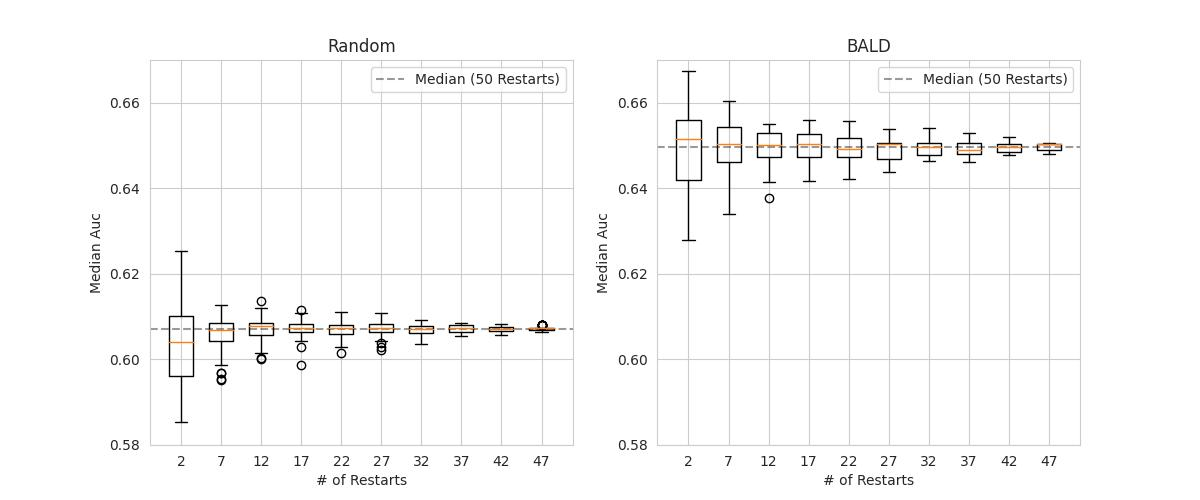
\includegraphics[width=\linewidth]{img/ablation_cifar_restarts}
    \caption{Created by the protocol described in Sec. \ref{sec:evaluation} for the Encoded Cifar10 dataset, with the classifier being trained from scratch. We observe similar characteristics, where a low number of restarts leads to extreme variance in the reported results.}
\end{figure}

\section{Oracle Curve Forecasting}\label{app:oracle_forecasting}
TODO

\section{Hyperparameters per AL Algorithm}\label{app:agent_hyperparameters}
\begin{table}[H]
    \caption{Selected hyperparameters for all tested acquisition functions. Last column indicates the source of our implementation.}
	\centering
	\begin{tabular}{l || l | l | l}
		Algorithm & \makecell{Sample\\Size} & Other & Source\\
		\hline
		BADGE & 100 & & Based on \cite{ashdeep, curelab}\\
		BALD & 100 & Dropout Trials: 5 & Based on \cite{pycls} \\
		Coreset & 8000 & & Own \\
		TypiClust & 10000 & \makecell[tl]{Min Cluster Size: 5\\Max \# Clusters: 500} & Based on \cite{hacohen2022active} \\
		Margin & 8000 & & Own\\
		Entropy & 8000 &  & Own\\
	\end{tabular}
\end{table}

\section{Hyperparameters and Preprocessing per Dataset}\label{app:hyperparameters}
For all our datasets we use the pre-defined train/test splits, if given. 
In the remaining cases, we define test sets upfront and store them into separate files to keep them fixed across all experiments.
The validation set is split in the experiment run itself and depends on the dataset-seed.\\
\textbf{Tabular:}
We use \textbf{Splice}, \textbf{DNA} and \textbf{USPS} from LibSVMTools \cite{libsvmtools}.
All three datasets are normalized between [0, 1]. \\
\textbf{Image:}
We use \textbf{FashionMNIST} \cite{xiao2017fashion} and \textbf{Cifar10} \cite{krizhevsky2009learning}, since both are widely used in AL literature.
Both datasets are normalized according to their standard protocols. \\
\textbf{Text:}
We use \textbf{News Category} \cite{misra2022news} and \textbf{TopV2} \cite{chen-etal-2020-low-resource}.
For News Category we use  the 15 most common categories as indicated by its Kaggle site.
We additionally drop sentences above 80 words to reduce the padding needed (retaining 99,86\% of the data).
For TopV2, we are only using the "alarm" domain.
Both datasets are encoded with pre-trained GloVe (Common Crawl 840B Tokens) embeddings \cite{pennington2014glove}.
Since neither dataset provided a fixed test set, we randomly split 7000 datapoints into a test set.
%
\begin{table}[H]
	\centering
	\begin{tabular}{l || l l l }
		Dataset & Seed Set & Budget & Val Split \\
		\hline
		Splice & 1 & 400 & 0.2 \\
		SpliceEnc. & 1 & 60 & 0.2 \\
		DNA & 1 & 300 & 0.2 \\
		DNAEnc & 1 & 40 & 0.2 \\
		USPS & 1 & 400 & 0.2 \\
		USPSEnc & 1 & 600 & 0.2 \\
		FashionMnist & 100 & 2000 & 0.04 \\
		FashionMnistEnc & 1 & 500 & 0.04 \\
		Cifar10 & 100 & 2000 & 0.04  \\
		Cifar10Enc & 1 & 350 & 0.04  \\
		TopV2 & 1 & 125 & 0.25  \\
		News & 1 & 1500 & 0.03  \\
	\end{tabular}
	\caption{Size of the seed set is given by number of labeled sample per class.}
	\label{tab:architecture_hps}
\end{table}
\begin{table}[H]
\centering
\begin{tabular}{l || l | l l l l l}
	Dataset & Classifier & Optimizer & LR & Weight Decay & Dropout & Batch Size \\
	\hline
	Splice & [24, 12] & NAdam & 1.2e-3 & 5.9e-5 & 0 & 43 \\
	SpliceEnc. & linear & NAdam & 6.2e-4 & 5.9e-6 & 0 & 64 \\
	DNA & [24, 12] & NAdam & 3.9e-2 & 3.6e-5 & 0 & 64 \\
	DNAEnc & linear & NAdam & 1.6e-3 & 4e-4 & 0 & 64 \\
	USPS & [24, 12] & Adam & 8.1e-3 & 1.5e-6 & 0 & 43 \\
	USPSEnc & linear & NAdam & 7.8e-3 & 1.9e-6 & 0 & 64 \\
	FashionMnist & ResNet18 & NAdam & 1e-3 & 0 & 0 & 64 \\
	FashionMnistEnc & linear & Adam & 1.6e-3 & 1e-5 & 5e-2 & 64 \\
	Cifar10 & ResNet18 & NAdam & 1e-3 & 0 & 0 & 64 \\
	Cifar10Enc & linear & NAdam & 1.7e-3 & 2.3e-5 & 0 & 64 \\
	TopV2 & BiLSTM & NAdam & 1.5e-3 & 1.7e-7 & 5e-2 & 64 \\
	News & BiLSTM & NAdam & 1.5e-3 & 1.7e-7 & 5e-2 & 64 \\
\end{tabular}
\caption{Classifier architectures and optimized hyperparameters per dataset. Numbers in brackets signify a MLP with corresponding hidden layers.}
\label{tab:architectures}
\end{table}

\section{AL Pseudocode}\label{app:pseudocode}
\begin{algorithm}[H]
	\caption{Active Learning Loop}\label{alg:active_learning}
	\begin{algorithmic}[1]
		\Require $\LL, \U, \D_\text{test}, \operatorname{Train}, \operatorname{Seed}, \hat y$
		\Require $\Omega$ \Comment{Acquisition Function}
		\State $\LL^{(1)} \gets \operatorname{Seed}(\U)$  \Comment{Create the initial labeled set}
		\State $\U^{(1)} \gets \U$
		\For{$i := 1 \ldots B$}
		\State $\text{acc}^{(i)} \gets \operatorname{Train}(\LL^{(i)})$ 
		\State $a^{(i)} \gets \Omega(\mathcal{U}^{(i)})$ 
		\State $\mathcal{L}^{(i+1)} \gets \mathcal{L}^{(i)} \cup \{(\U^{(i)}_a, A(\U^{(i)}_{a}))\}$
		\State $\U^{(i+1)} \gets \U^{(i)} \setminus \{\U^{(i)}_a\}$
		\EndFor
		\State
		\Return $\frac{1}{B} \sum_{i=1}^{B} \text{acc}^{(i)}$
	\end{algorithmic}
\end{algorithm}

\begin{algorithm}[H]
	\caption{Retrain}\label{alg:retrain}
	\begin{algorithmic}[1]
		\Require $\LL, \D_\text{val}, \D_\text{test}$
		\Require $\hat y, e_\text{max}$
		\State $\text{loss}^* \gets \infty$
		\For{$i := 1 \ldots e^{\text{max}}$}
		\State $\hat y_{i+1} \gets \hat y_i - \eta \nabla_{\hat y} \ell(\mathcal{L}, \hat y)$
		\State $\text{loss}_i \gets \ell(\mathcal{D}^\text{val}, \hat y)$
		\If{$\text{loss}_i < \text{loss}^*$}
		\State $\text{loss}^* \gets \text{loss}_i$
		\Else
		\State Break
		\EndIf
		\EndFor
		\State
		\Return Acc($\mathcal{D}^\text{test}, \hat y$)
	\end{algorithmic}
\end{algorithm}

\begin{algorithm}[H]
\caption{Acquire Oracle $\Omega$}\label{alg:oracle}
\begin{algorithmic}[1]
    \Require $\mathcal{U}, \mathcal{L}, A, \mathcal{D}_\text{test}, \tau, \hat y_\theta$ 
    \Require Train, Margin, Acc
    \State $\text{acc}^0 \gets \text{acc}^* \gets \operatorname{Acc}(\mathcal{D}_\text{test}, \hat y_\theta)$ 
    \For{$k := 1 \ldots \tau$}
        \State $u_k = \operatorname{unif}(\U)$
    \State $\mathcal{L}' \gets \mathcal{L}^{(i)} \cup \{(u_k, A(u_k))\}$
    \State $\hat y'_\theta \gets \operatorname{Train}(\mathcal{L}', \hat y_\theta)$
        \State $\text{acc}' \gets \text{Acc}(\D_\test, \hat y'_\theta)$
    %\State $r \gets \text{acc}' - \text{acc}$
    \If{$\text{acc}' > \text{acc}^*$} 
    \State $\text{acc}^* \gets \text{acc}'$
    \State $u^* \gets u_k$
    \EndIf
    \EndFor
    \If{$\text{acc}^0 = \text{acc}^*$}
    \State $u^* \gets \operatorname{Margin}(\mathcal{U}, \hat y_\theta)$
    \EndIf
    \Return $u^*$
\end{algorithmic}
\end{algorithm}
Alg. \ref{alg:oracle} replaces the acquisition function $\Omega$ in the AL loop (Alg. \ref{app:pseudocode} line 5). 
 
\end{document}
